\kmuttchapter{RESULT AND DISCUSSION}
%section 1: Asymmetric tunneling
We start by investigating the tunneling properties of electron across tilted Dirac cone heterojunctions where we focus on how
the effect of the gate potential and tilt affect the electron transmission.  
%section 2: Measure the tilted strength 
%we focused on the tilted parameter $w_0$ since it is the parameter that determines the character of the Dirac cone.
Then, we demonstrate a method to measure the tilted strength of the Dirac cone by identifying the tunneling behavior.
%section 3 Pseudo magnetic field
Finally, we show that the transport behaviors of electron in tilted Dirac cone material are analogous to electron under
the influence of magnetic field. We also show the derivation of magnetic field strength as a function of gate potential and tilted parameter.


The calculation of transmission probability is carried out using Eq. \ref{eq:tp}
%In this study, we assumed that the system is in a condensed state, where the thermal noise can be neglected
\section{Angular dependent of transmission probability} \label{sec:asym}
    The transmission probabilities across the tilted Dirac cone heterojunctions under the variation of gate potential are presented in Fig. \ref{fig:asym}.
    The transmission profiles are symmetric in the case of $w_0 = 0$ regardless of the gate potential. 
    When the tilted parameter is non-zero, the transmission profiles are shifted along the direction of the tilt and consequently become asymmetric, where the magnitude of the shift depends on the tilted strength of the Dirac cone.
    However, the present of the tilt barely affects the tunneling profiles when the applied gate potential is close to the Fermi energy as shown in Fig. \ref{fig:asym2}.
    This is because the Fermi surface is small and the allowed wavevector states are narrowed. Therefore, electron propagations other than the normal incident are backscattered.\\
    
    Interestingly, when the applied gate voltage $U$ is larger than the Fermi energy $E_F$, the transmission profiles exhibit peak tunneling as shown in Fig. \ref{fig:asym3}-\subref{fig:asym4}.
    These kind of tunnelings are called resonant tunneling, which occurred when the condition $q_x L = n \pi$, $n = 0, \pm1,...$ in Eq. \ref{eq:tp} is met.
    %In addition, the normal incident perfect tunneling is not affected by the transverse tilted Dirac cone.
    
    \begin{figure}[H] %Asymmetric tunneling
        \centering
        \begin{subfigure}[b]{0.3\linewidth}
            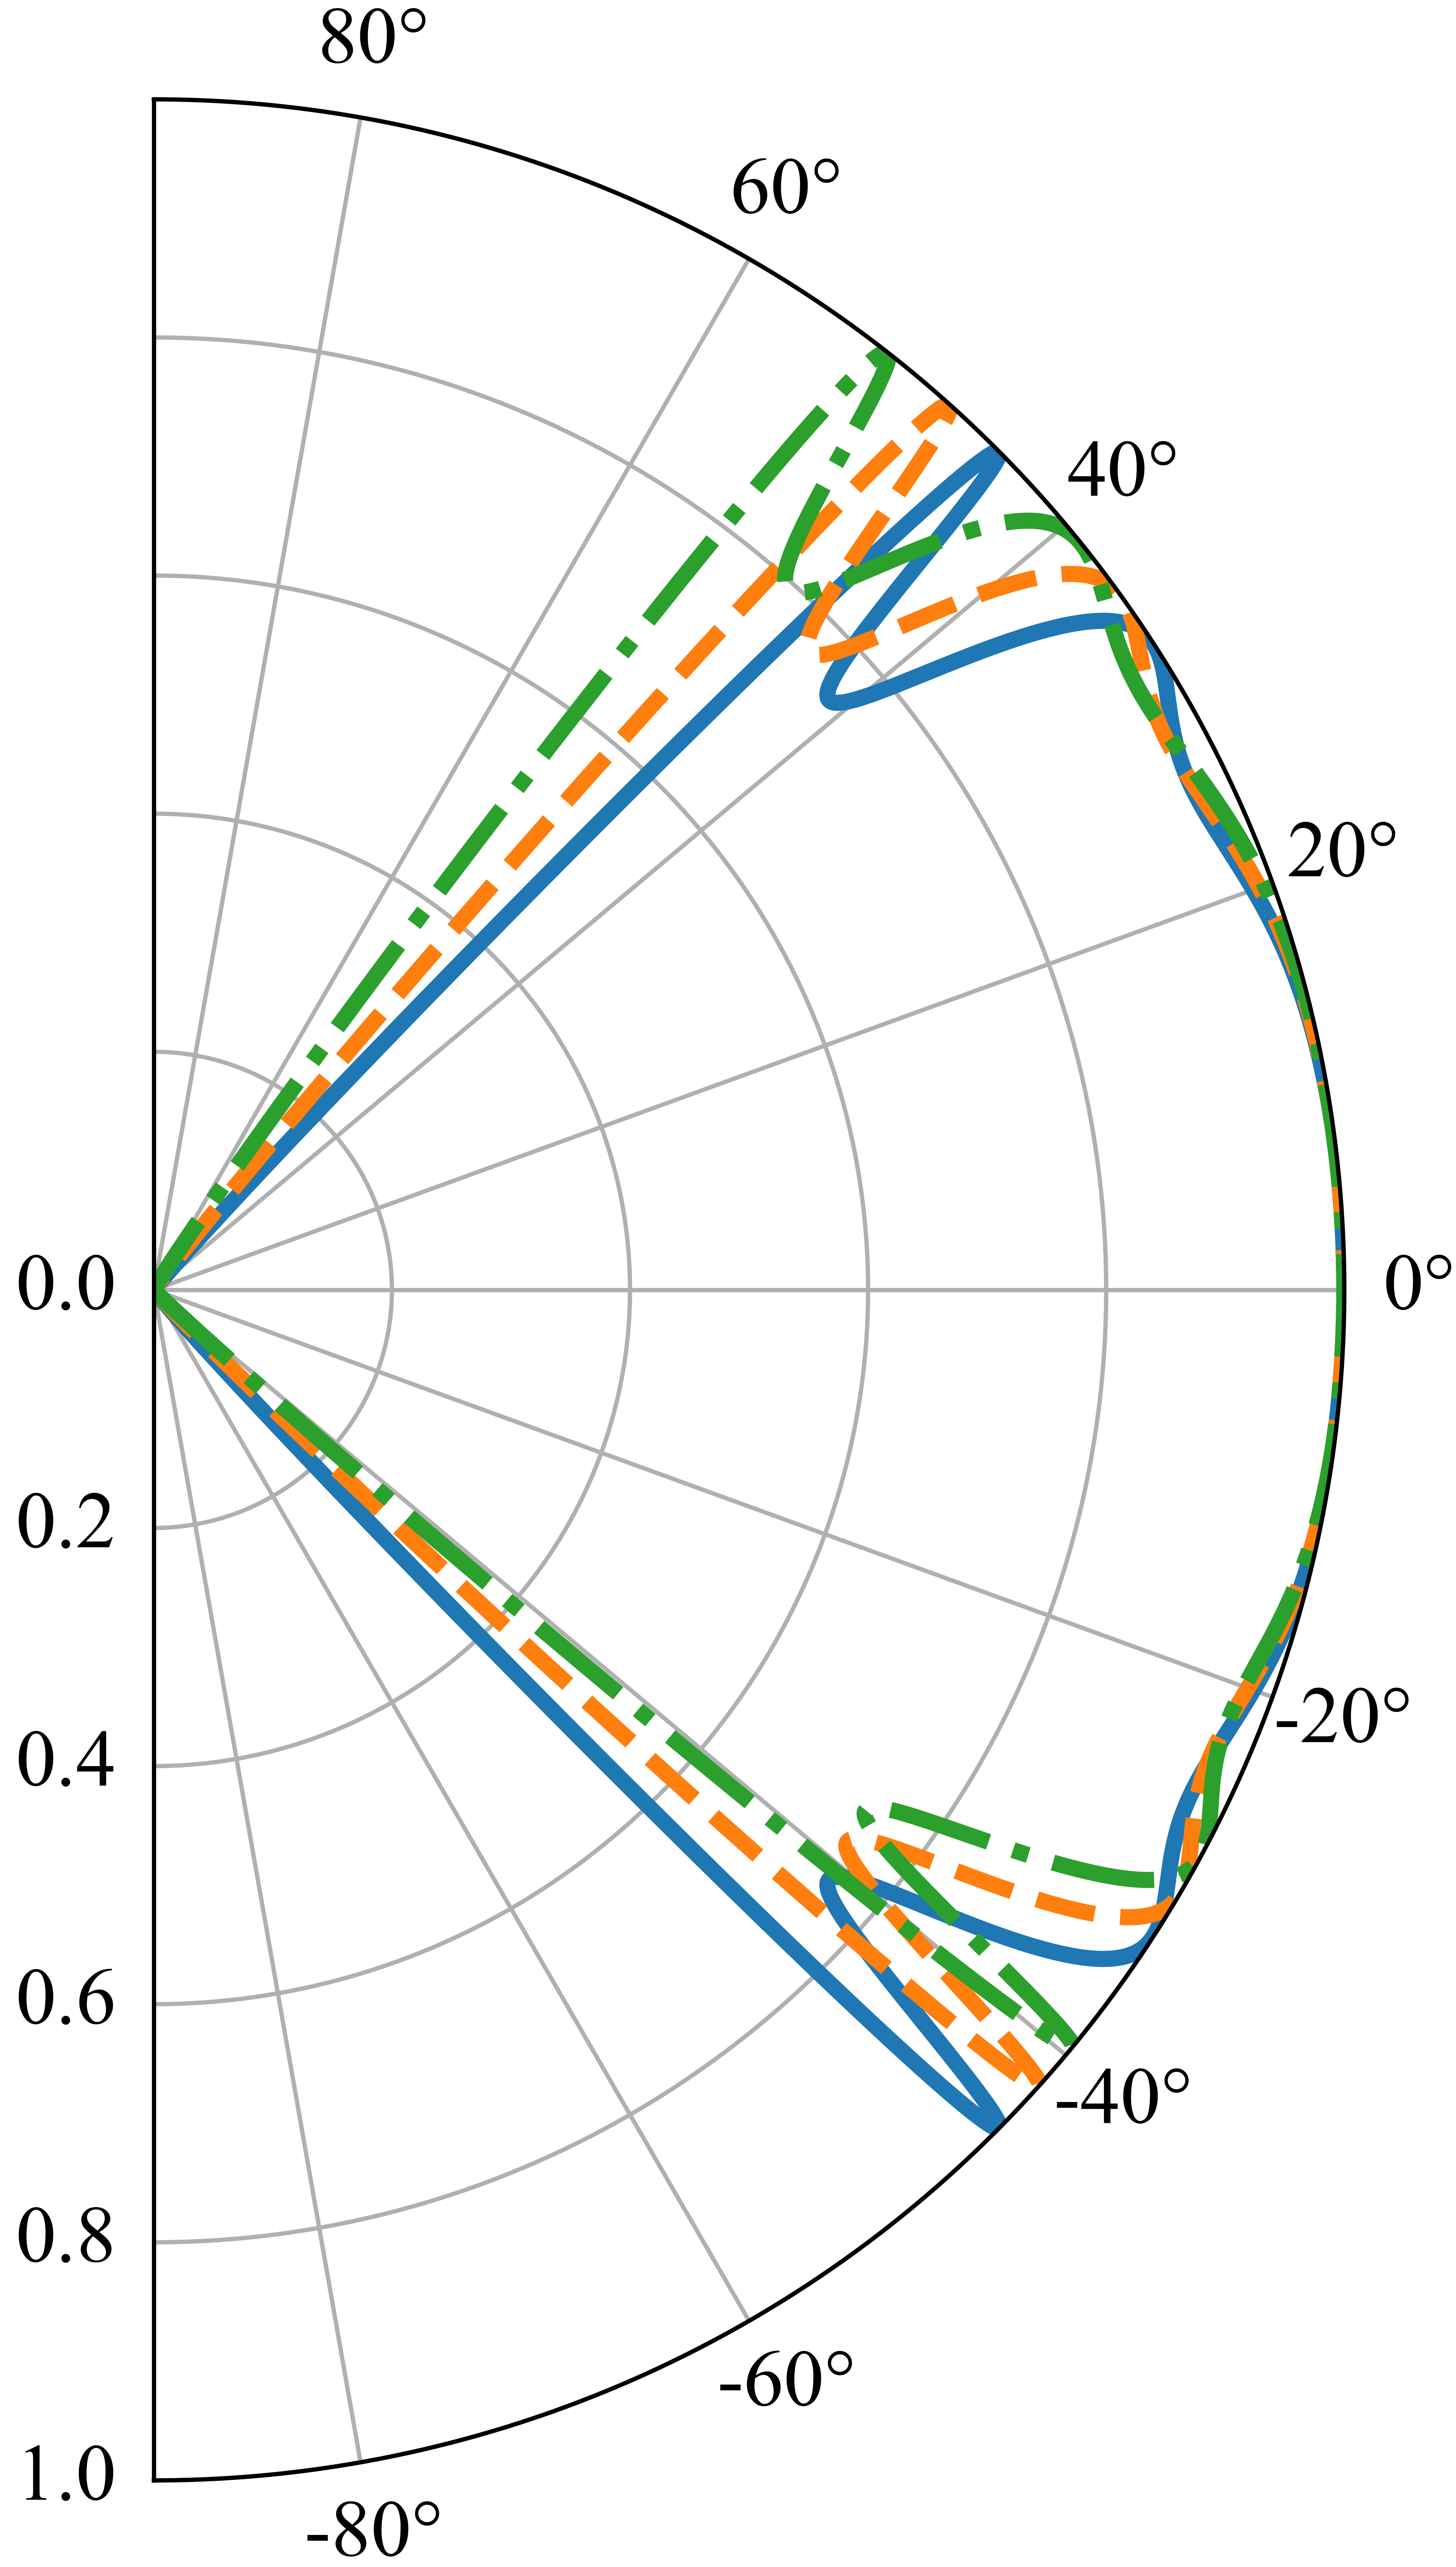
\includegraphics[width=\linewidth]{fig/tunneling shift/U0.02.png}
            \caption{}
            \label{fig:asym1}
        \end{subfigure}
        \begin{subfigure}[b]{0.3\linewidth}
            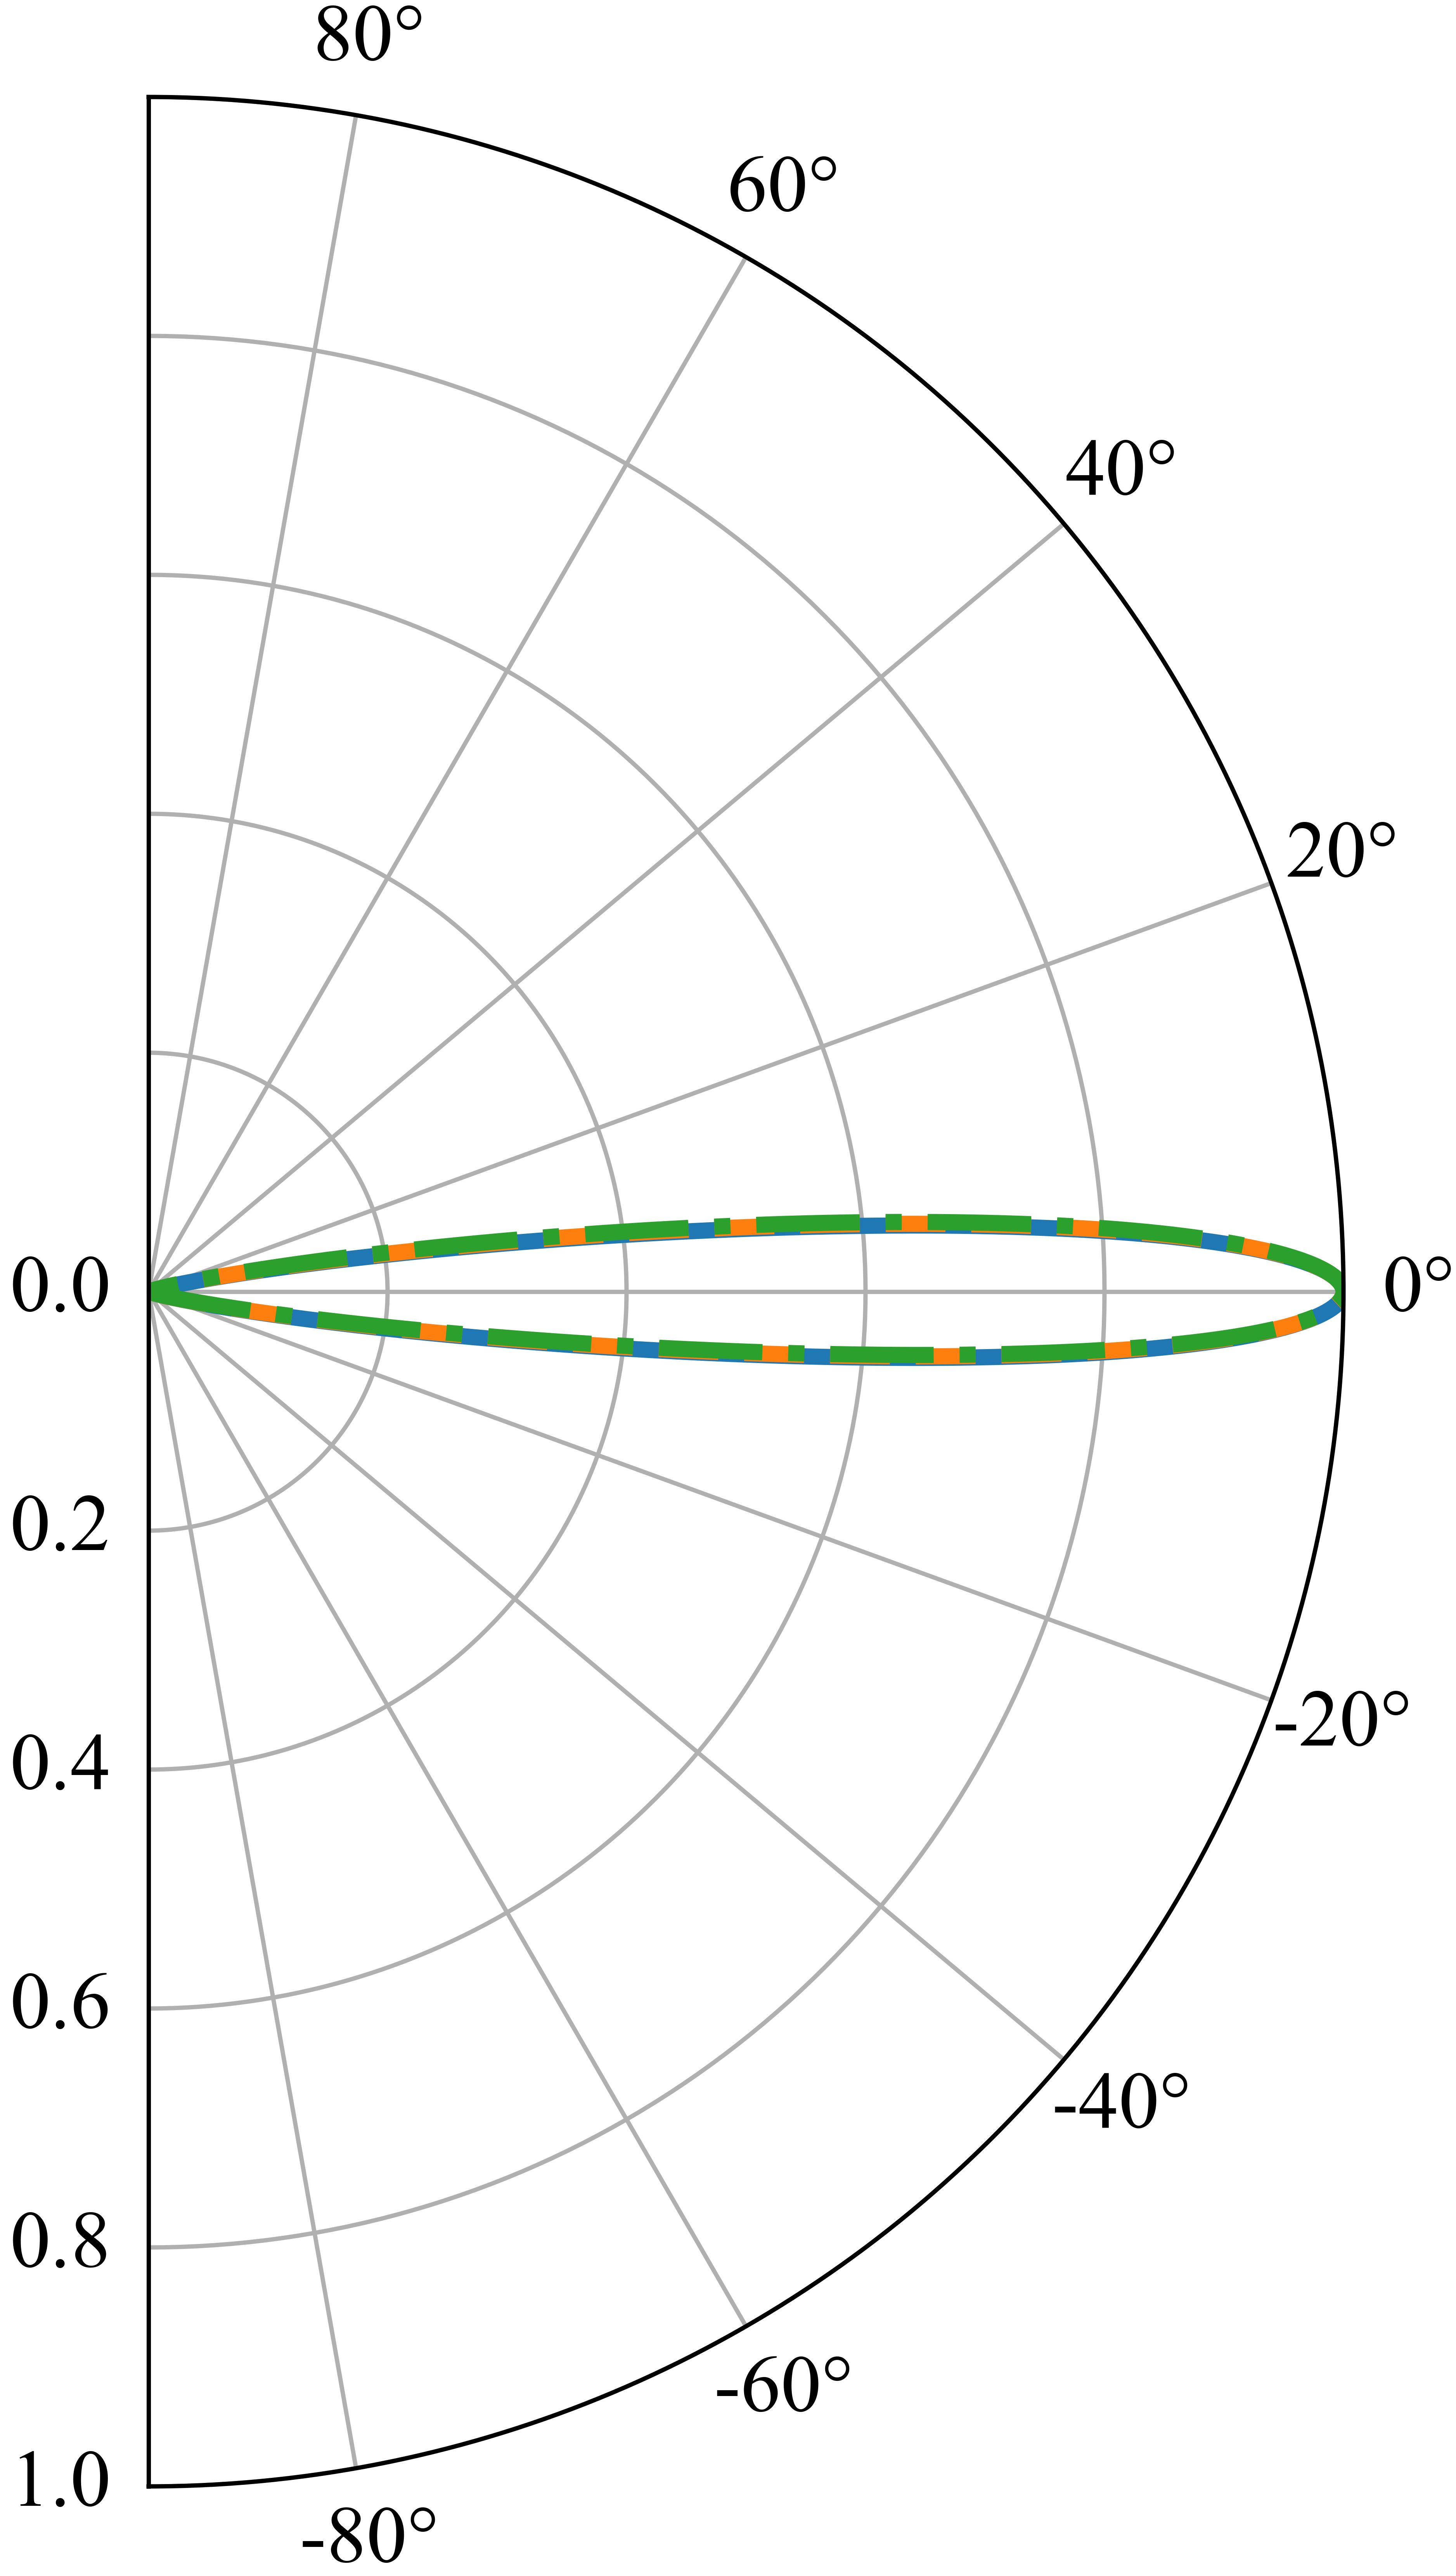
\includegraphics[width=\linewidth]{fig/tunneling shift/U0.07.png}
            \caption{}
            \label{fig:asym2}
        \end{subfigure}

        \begin{subfigure}[b]{0.3\linewidth}
            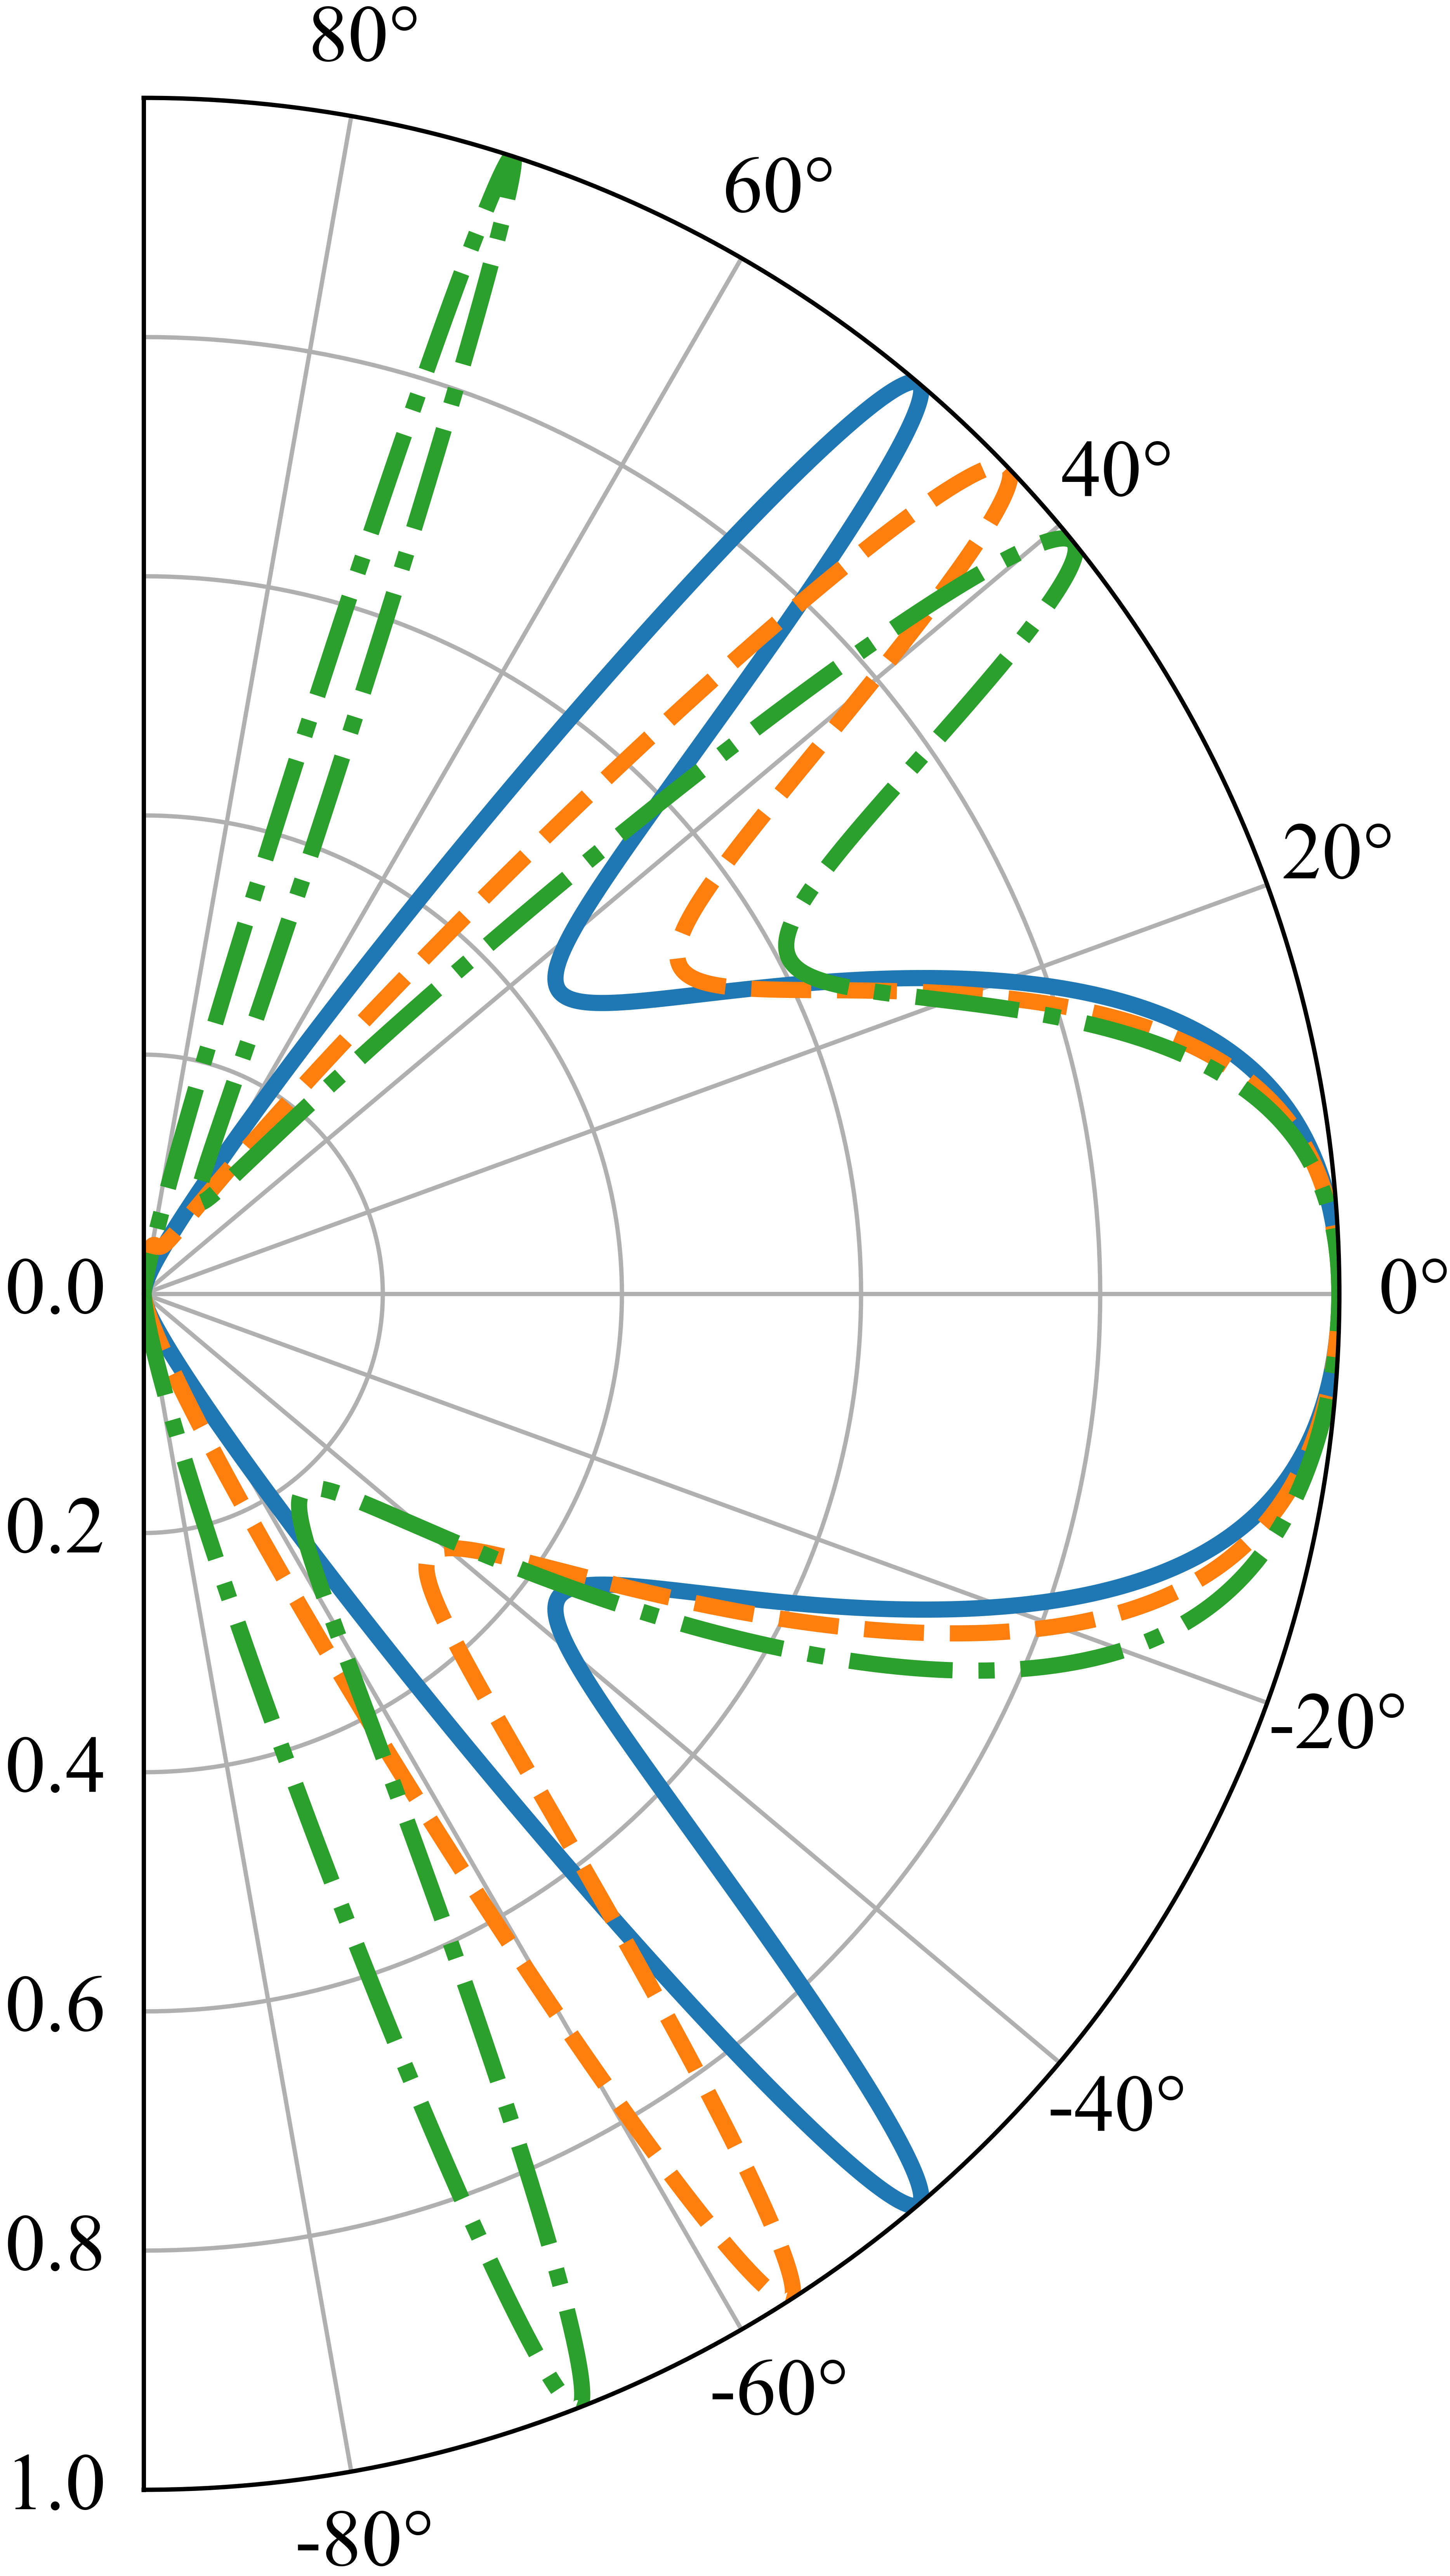
\includegraphics[width = \linewidth]{fig/tunneling shift/U0.2.png}
            \caption{}
            \label{fig:asym3}
        \end{subfigure}
        \begin{subfigure}[b]{0.3\linewidth}
            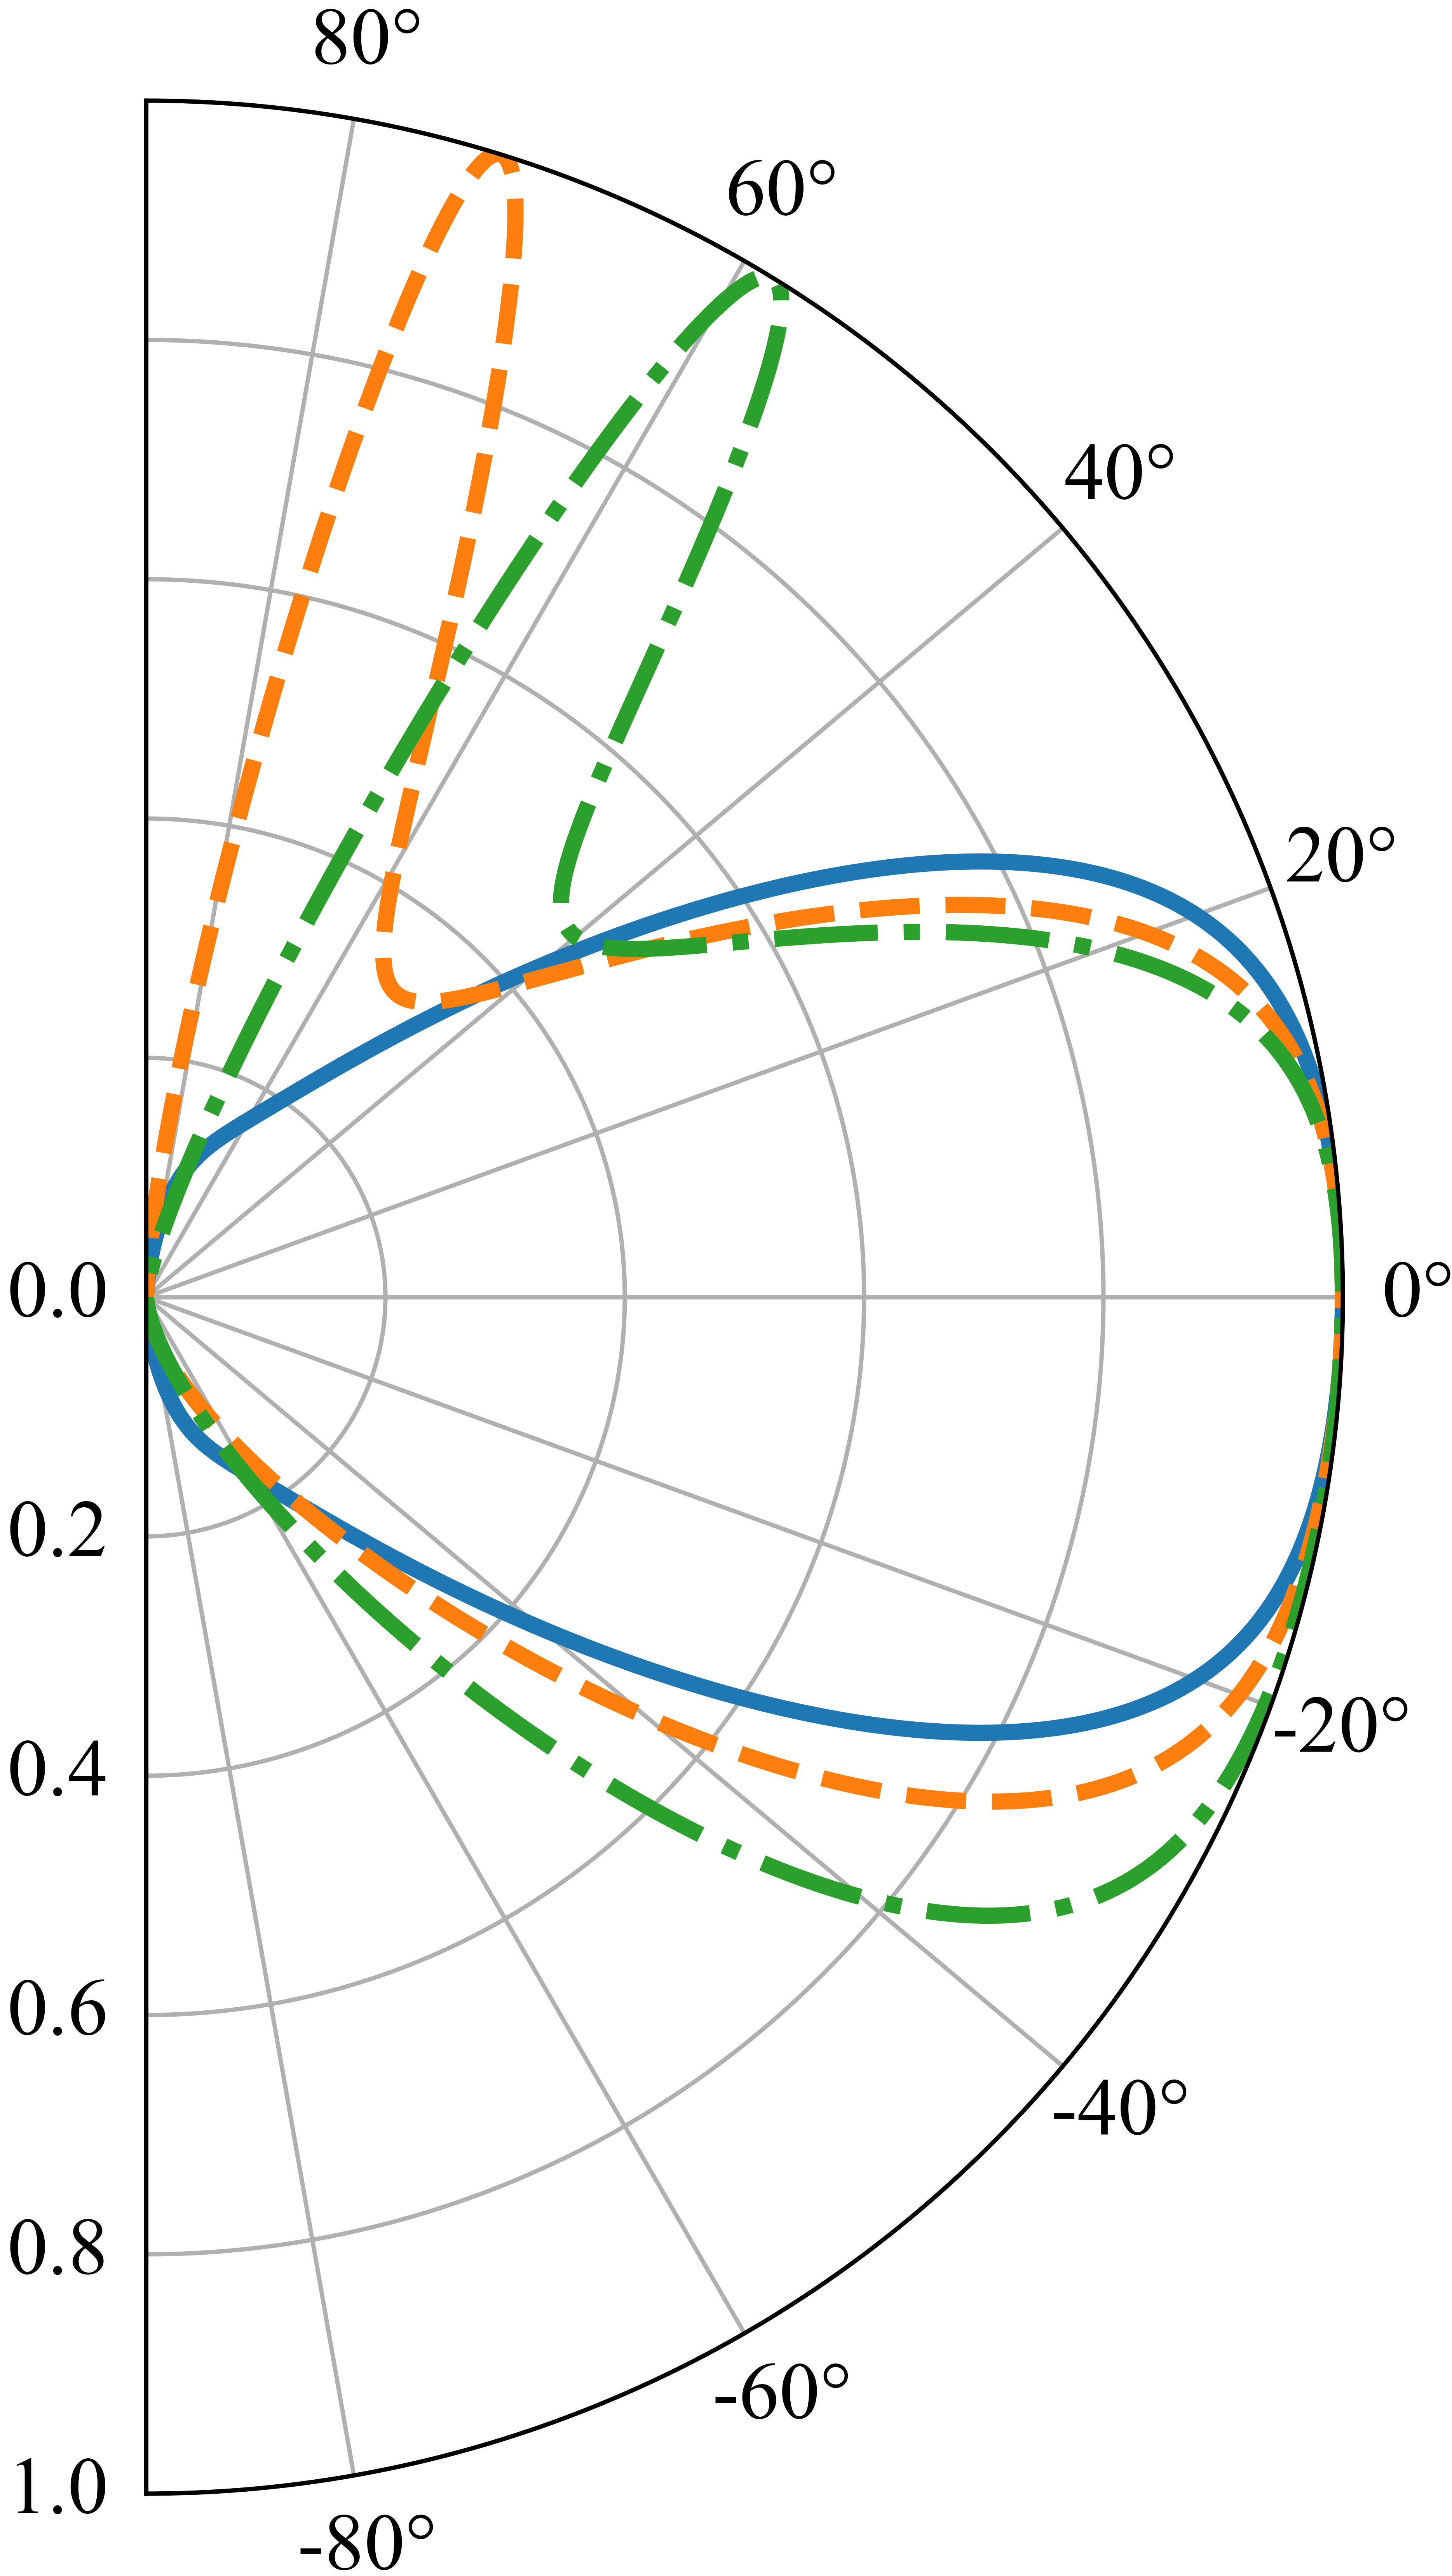
\includegraphics[width = \linewidth]{fig/tunneling shift/U0.285.png}
            \caption{}
            \label{fig:asym4}
        \end{subfigure}
        \caption{The same cup of coffee. Two times.}
        \label{fig:asym}
    \end{figure}

\section{The tilted strength identification by means of the tunneling resonance properties} \label{sec:find w}
    The resonant tunnelings are arisen if the given $U, E_F$ and, $w_0$ satisfy the resonance condition.
    Modulating these parameters result in shifting of resonant tunneling angles as previously reported in section \ref{sec:asym}.
    In this section, we demonstrate that by measuring the asymmetric resonant tunneling angles, the tilted parameter can be determined.
    Consider the resonance condition
    %by tracking how much those resonance conditions are shifted
    \begin{align} \label{eq:w0}
        L \sqrt{\left( \frac{E_F-U}{\hbar v_F}+ w_0 k_y \right)^2 -k_y^2} = n \pi \notag\\
        w_{0 \pm} = \frac{U-E_F}{\hbar v_F k \sin{\phi}}\mp \sqrt{1+\left(\frac{n \pi}{k L \sin{\phi}}\right)^2}
    \end{align}
    where subscript $+(-)$ satisfy the positive(negative) angle $\phi$ region.
    One can obtain the tilted parameter by applying the gate voltage and Fermi energy then measure the resonant tunneling angle, which can be experimentally observed
    by four-point probes technique \cite{Rahman2015}.
    To illustrate how to calculate for the tilted parameter, we substitute the configuration of dashed-dotted line in Fig. \ref{fig:asym3} to Eq. \ref{eq:w0}.
    We choose the resonance condition $n=4$, which corresponds to the resonant tunneling angle $\phi = 72^{\circ}$. We find $w_0 = 0.1$.\\
    
    However, this method is not at all practical since the variable $n$ is unlikely observable.
    Also, the only way to manipulate the electron propagations is by tuning the voltages through the bottom and top gate.
    In section \ref{sec:find w 2}, we propose a more practical method to identify the tilted strength, which again, involve with the resonant tunneling behaviors.

    %When the voltages are applied to the system, there will be 
    %For some given value of $U, E_F, \mathrm{and} $ 
    %resonance condition can be modulated by tuning $U, E_F$ and, $w_0$ since $q_x$ depends on these parameter. 
    %Electron propagations at normal incident undergo the Klein tunneling effect, where the transmission probability always equal to one.
    % the downside of this method is there are unknown parameter such as n
    %In the next section, we show how to get rid of n
\section{Oscillatory behavior of electron resonant tunneling}
    To understand the behaviors of resonant tunneling under the effect of the tilt and gate potential, 
    we plot the transmission probabilities at particular incident angle $\phi = 45^{\circ}$ shown in Fig. \ref{fig:tp 45 deg}.
    
    %the effect of the tilt does not destroy the uniformity of the oscillation, it simply shifted as the tilted parameter increased. 
    \begin{figure}[H]
        \centering
            \includegraphics[width=\linewidth]{fig/tp Ef = 0.08 e1 = 0 e2 = 0.05 e3 = 0.1.png}
            \caption{tp fixed angle}
        \label{fig:tp 45 deg}
    \end{figure}

\section{Revisit: The tilted strength identification by means of the tunneling resonance properties} \label{sec:find w 2}
    %This section we address the problem we have so for in section \ref{sec:find w}
    \begin{figure}[H] 
        \centering
        \begin{subfigure}[b]{0.45\linewidth}
            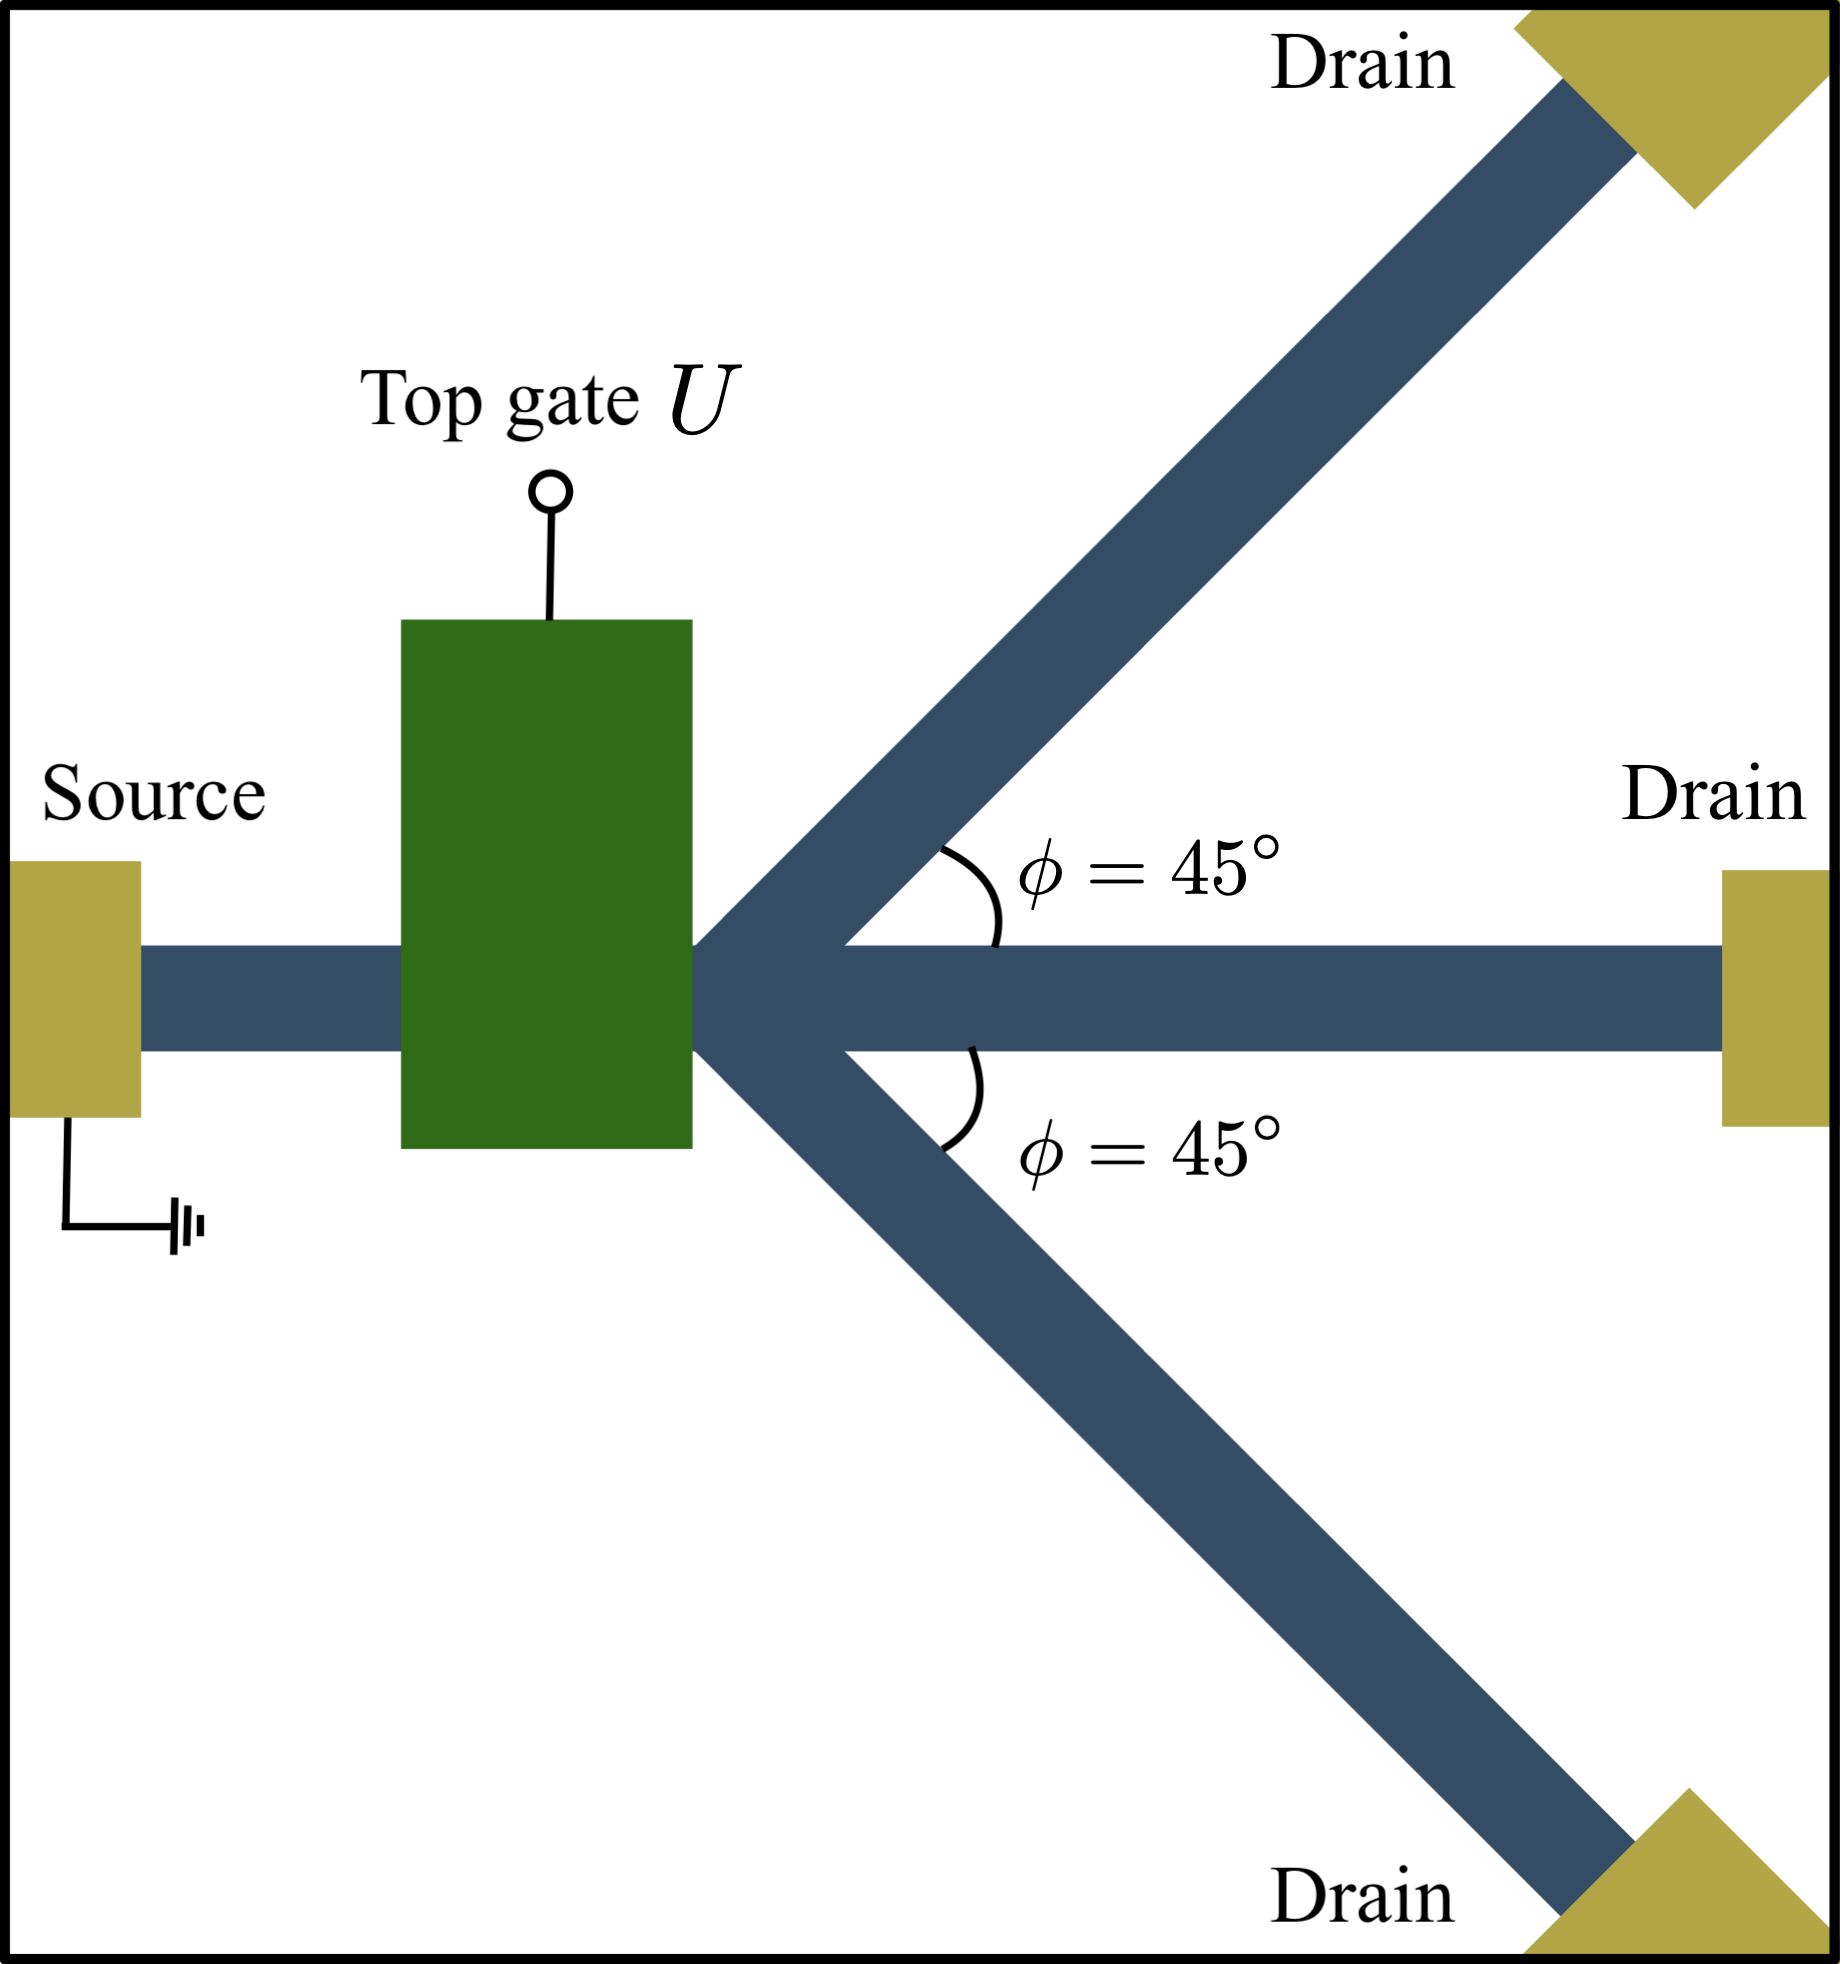
\includegraphics[width=\linewidth]{fig/3 arm structure.png}
            \caption{}
            \label{fig:3 arms}
        \end{subfigure}
        \begin{subfigure}[b]{0.3\linewidth}
            \includegraphics[width=\linewidth]{fig/tp Ef = 0.08 U1 = 0.1802 e1 = 0 e3 = 0.1.png}
            \caption{}
            \label{fig:tp at 45 deg}
        \end{subfigure}
        \caption{(a) The device structure for the measurement of resonant tunneling electron.  
                    Straight blue lines represent the transport region where both arms are $45^{\circ}$ angled with the normal direction. 
                    Green and yellow region represents top gate and electrode respectively. 
                    (b) Angular-dependent transmission for different applied voltages, U=180.2 meV for solid line and U=185.85 meV for dashed-dotted line. 
                    These voltages satisfy the resonance condition at $\phi = \frac{\pi}{4}$.}
        \label{fig:find w}
    \end{figure}
\section{Pseudo magnetic field} \label{sec:pseudo b}
    In section \ref{sec:asym}, we have shown that the tunneling behavior of electron across the tilted Dirac cone exhibits asymmetric transmission. 
    Previously, the transmission of this kind can be achieved by applying the magnetic barrier to the system \cite{RamezaniMasir2008,RamezaniMasir2010}.
    In this section, we demonstrate that the similar transmission profile can also be achieved in the tilted Dirac cone system without the magnetic barrier.
    Consider the x-component wavevector inside the barrier region $q_x = \sqrt{q^2-k_y^2}$, which can be rearranged into the form
    \begin{equation} \label{eq:k_shift}
        q_x \approx \sqrt{q'^2 -(k_y-q'w_0)^2}
    \end{equation} 
    where $q' = \frac{E_F-U}{\eta \hbar v_F}$. 
    Notice that the y-component wavevector in Eq. \ref{eq:k_shift} is shifted by the tilted Dirac cone similar to the wavevector shift by the effect of magnetic vector potential.
    Based on this analogy, we can derive the equivalent pseudo magnetic field
    \begin{align}
        -q' w_0 &= \frac{\xi}{l_B} \notag \\
        -\left(\frac{E_F-U}{\eta \hbar v_F}\right) w_0 &= \xi\sqrt{\frac{|e| B}{\hbar}} \notag \\
        B &= \left(\frac{\varepsilon w_0}{v_F}\right)^2 \frac{1}{\xi \gamma \hbar |e|}
    \end{align}
    where $\varepsilon = E_F-U$ is effective Fermi energy. 
    $\xi = \pm 1$ is in fact the direction of magnetic field, but since these fields are induced by the tilted Dirac cone, it can be considered as the direction of the tilt.
    The positive(negative) sign mean that the Dirac cone tilted to the left(right) side with respect to normal direction. 
    $\gamma = \pm 1$ indicate the carrier type in Fermi energy level.


   
\section{Transmission under the influence of pseudo magnetic field}
    To illustrate how pseudo magnetic field affects the tunneling behaviors compared to their real counterpart,
    the transmissions under the effect of pseudo and real magnetic fields are plotted as shown in Fig.\ref{fig:pseudo}.

    \begin{figure}[H] %Pseudo B field 
    \centering
        \begin{subfigure}[b]{0.3\linewidth}
            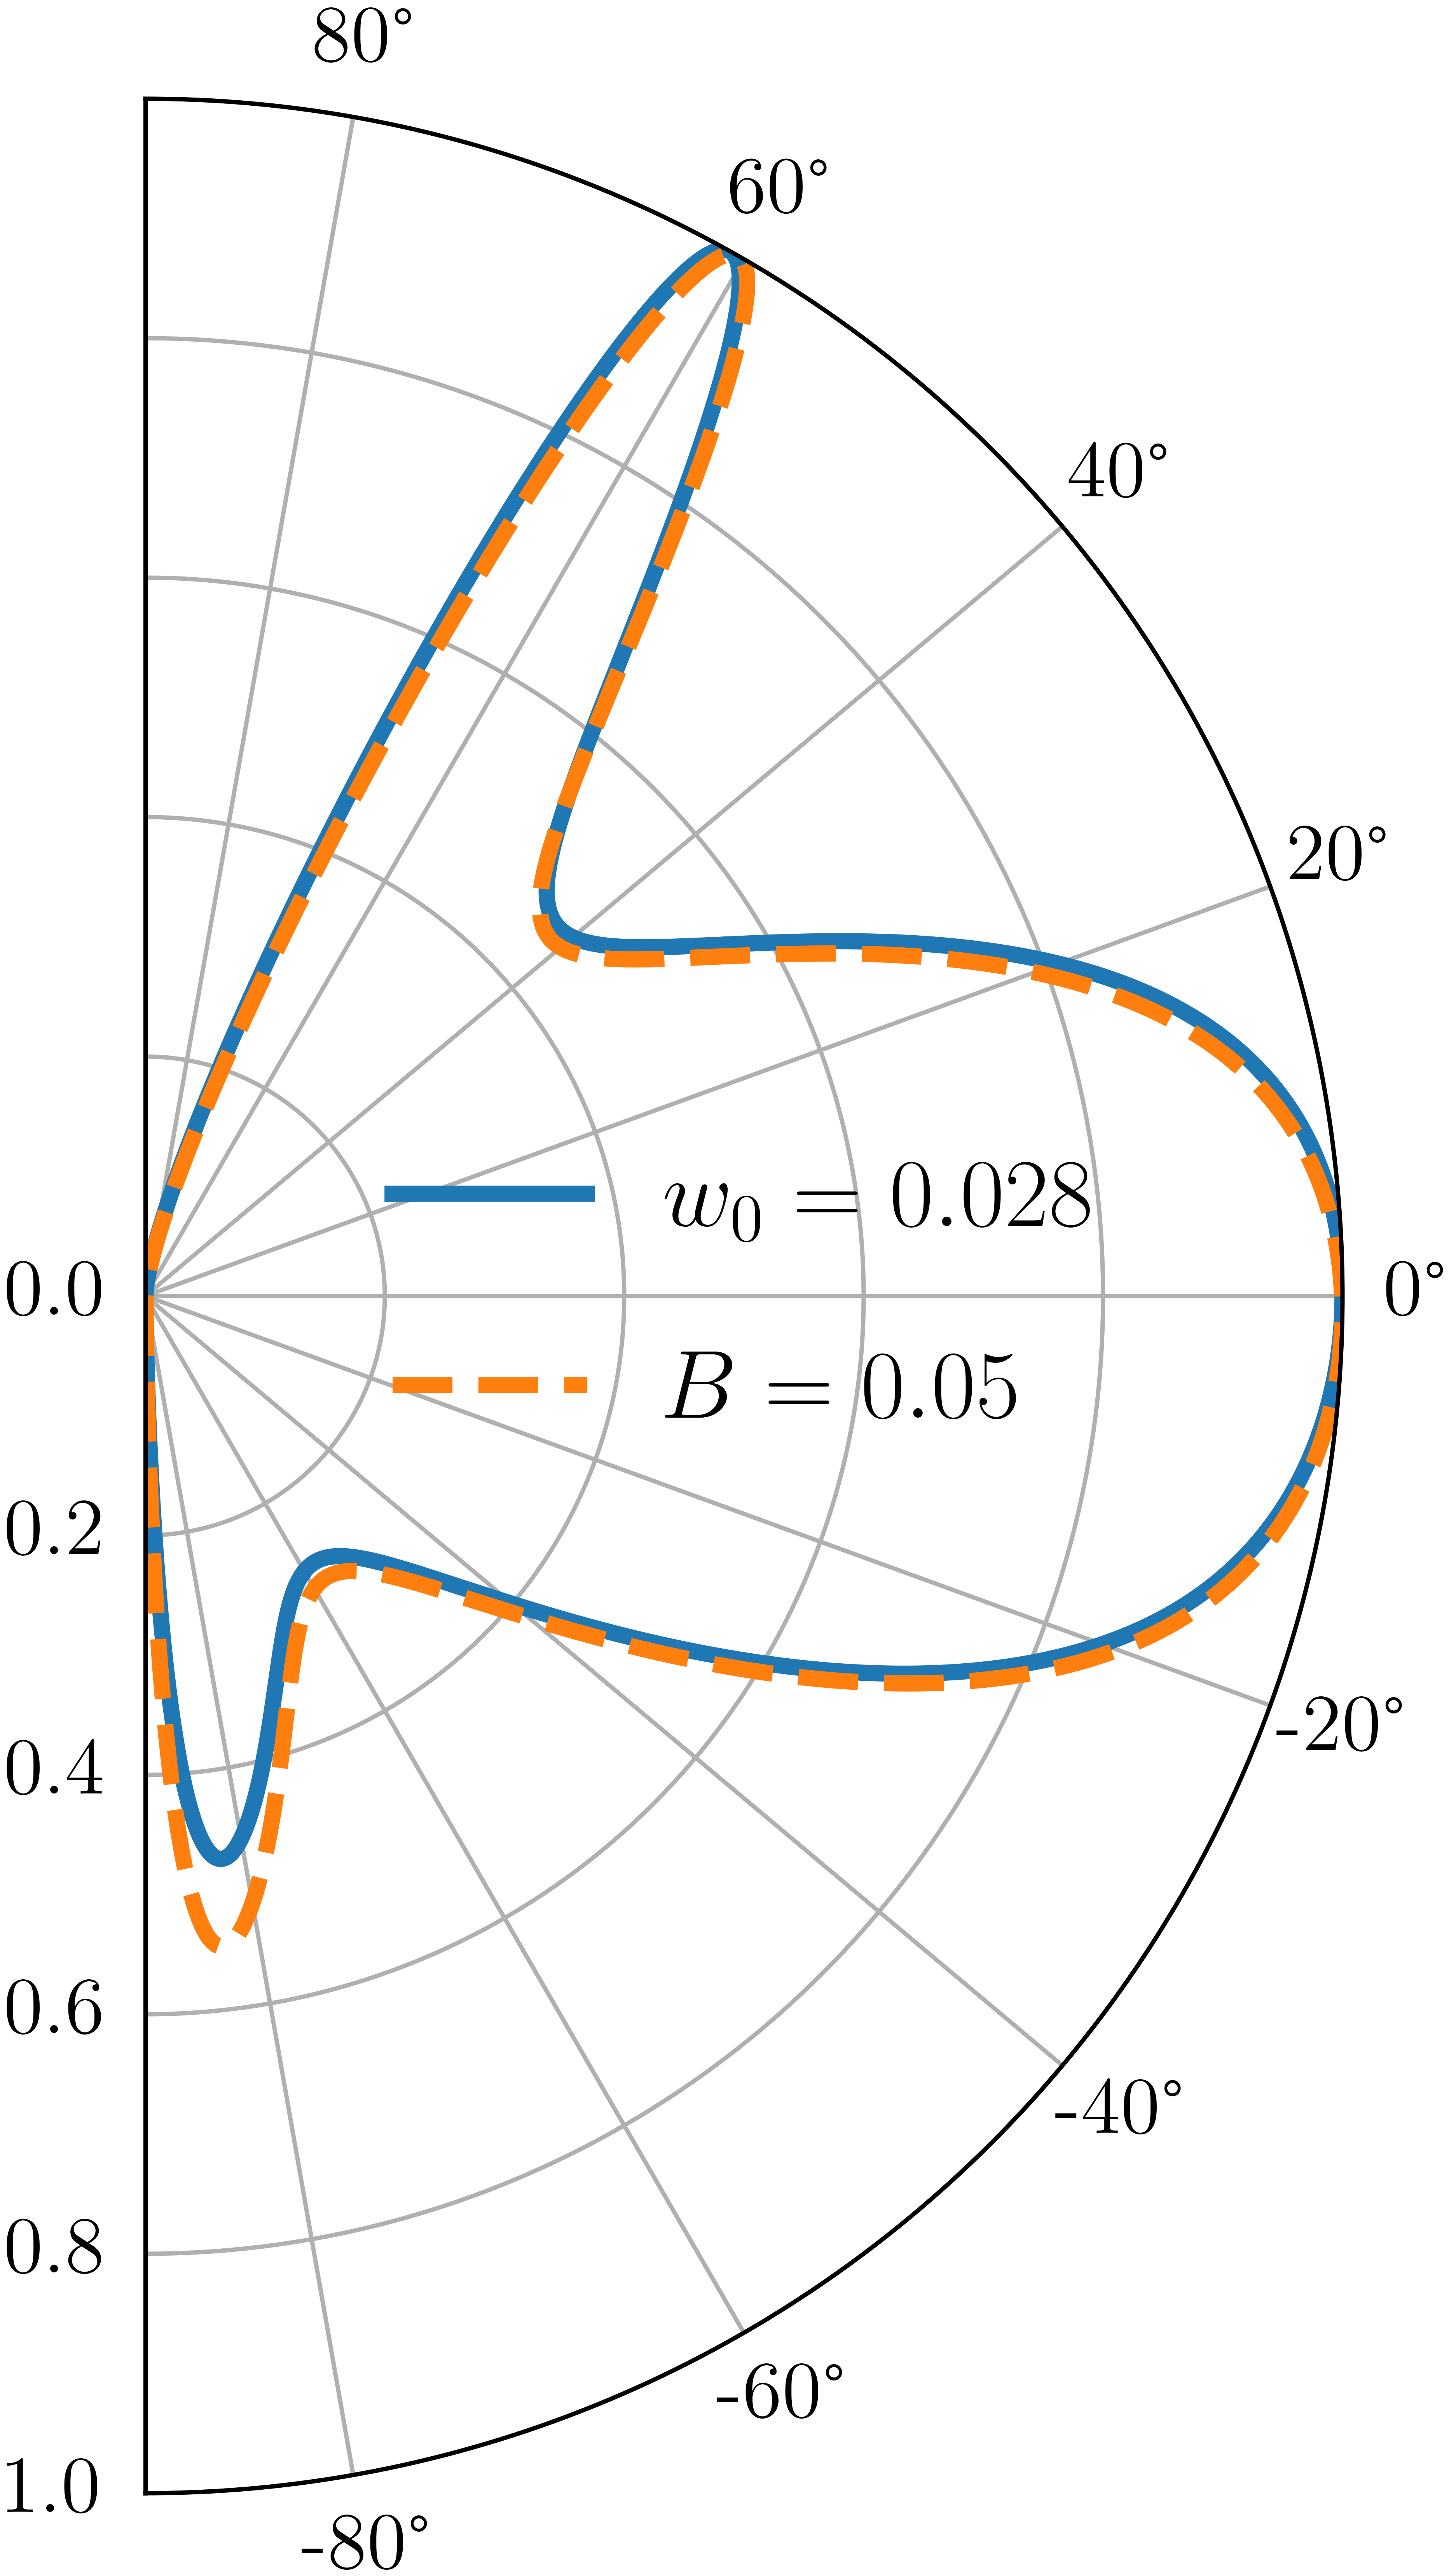
\includegraphics[width=\linewidth]{fig/pseudo B field/Ef0.0832 U0.285 B0.05 w0.028.png}
            \caption{}
            \label{fig:pseudo1}
        \end{subfigure}
        \begin{subfigure}[b]{0.3\linewidth}
            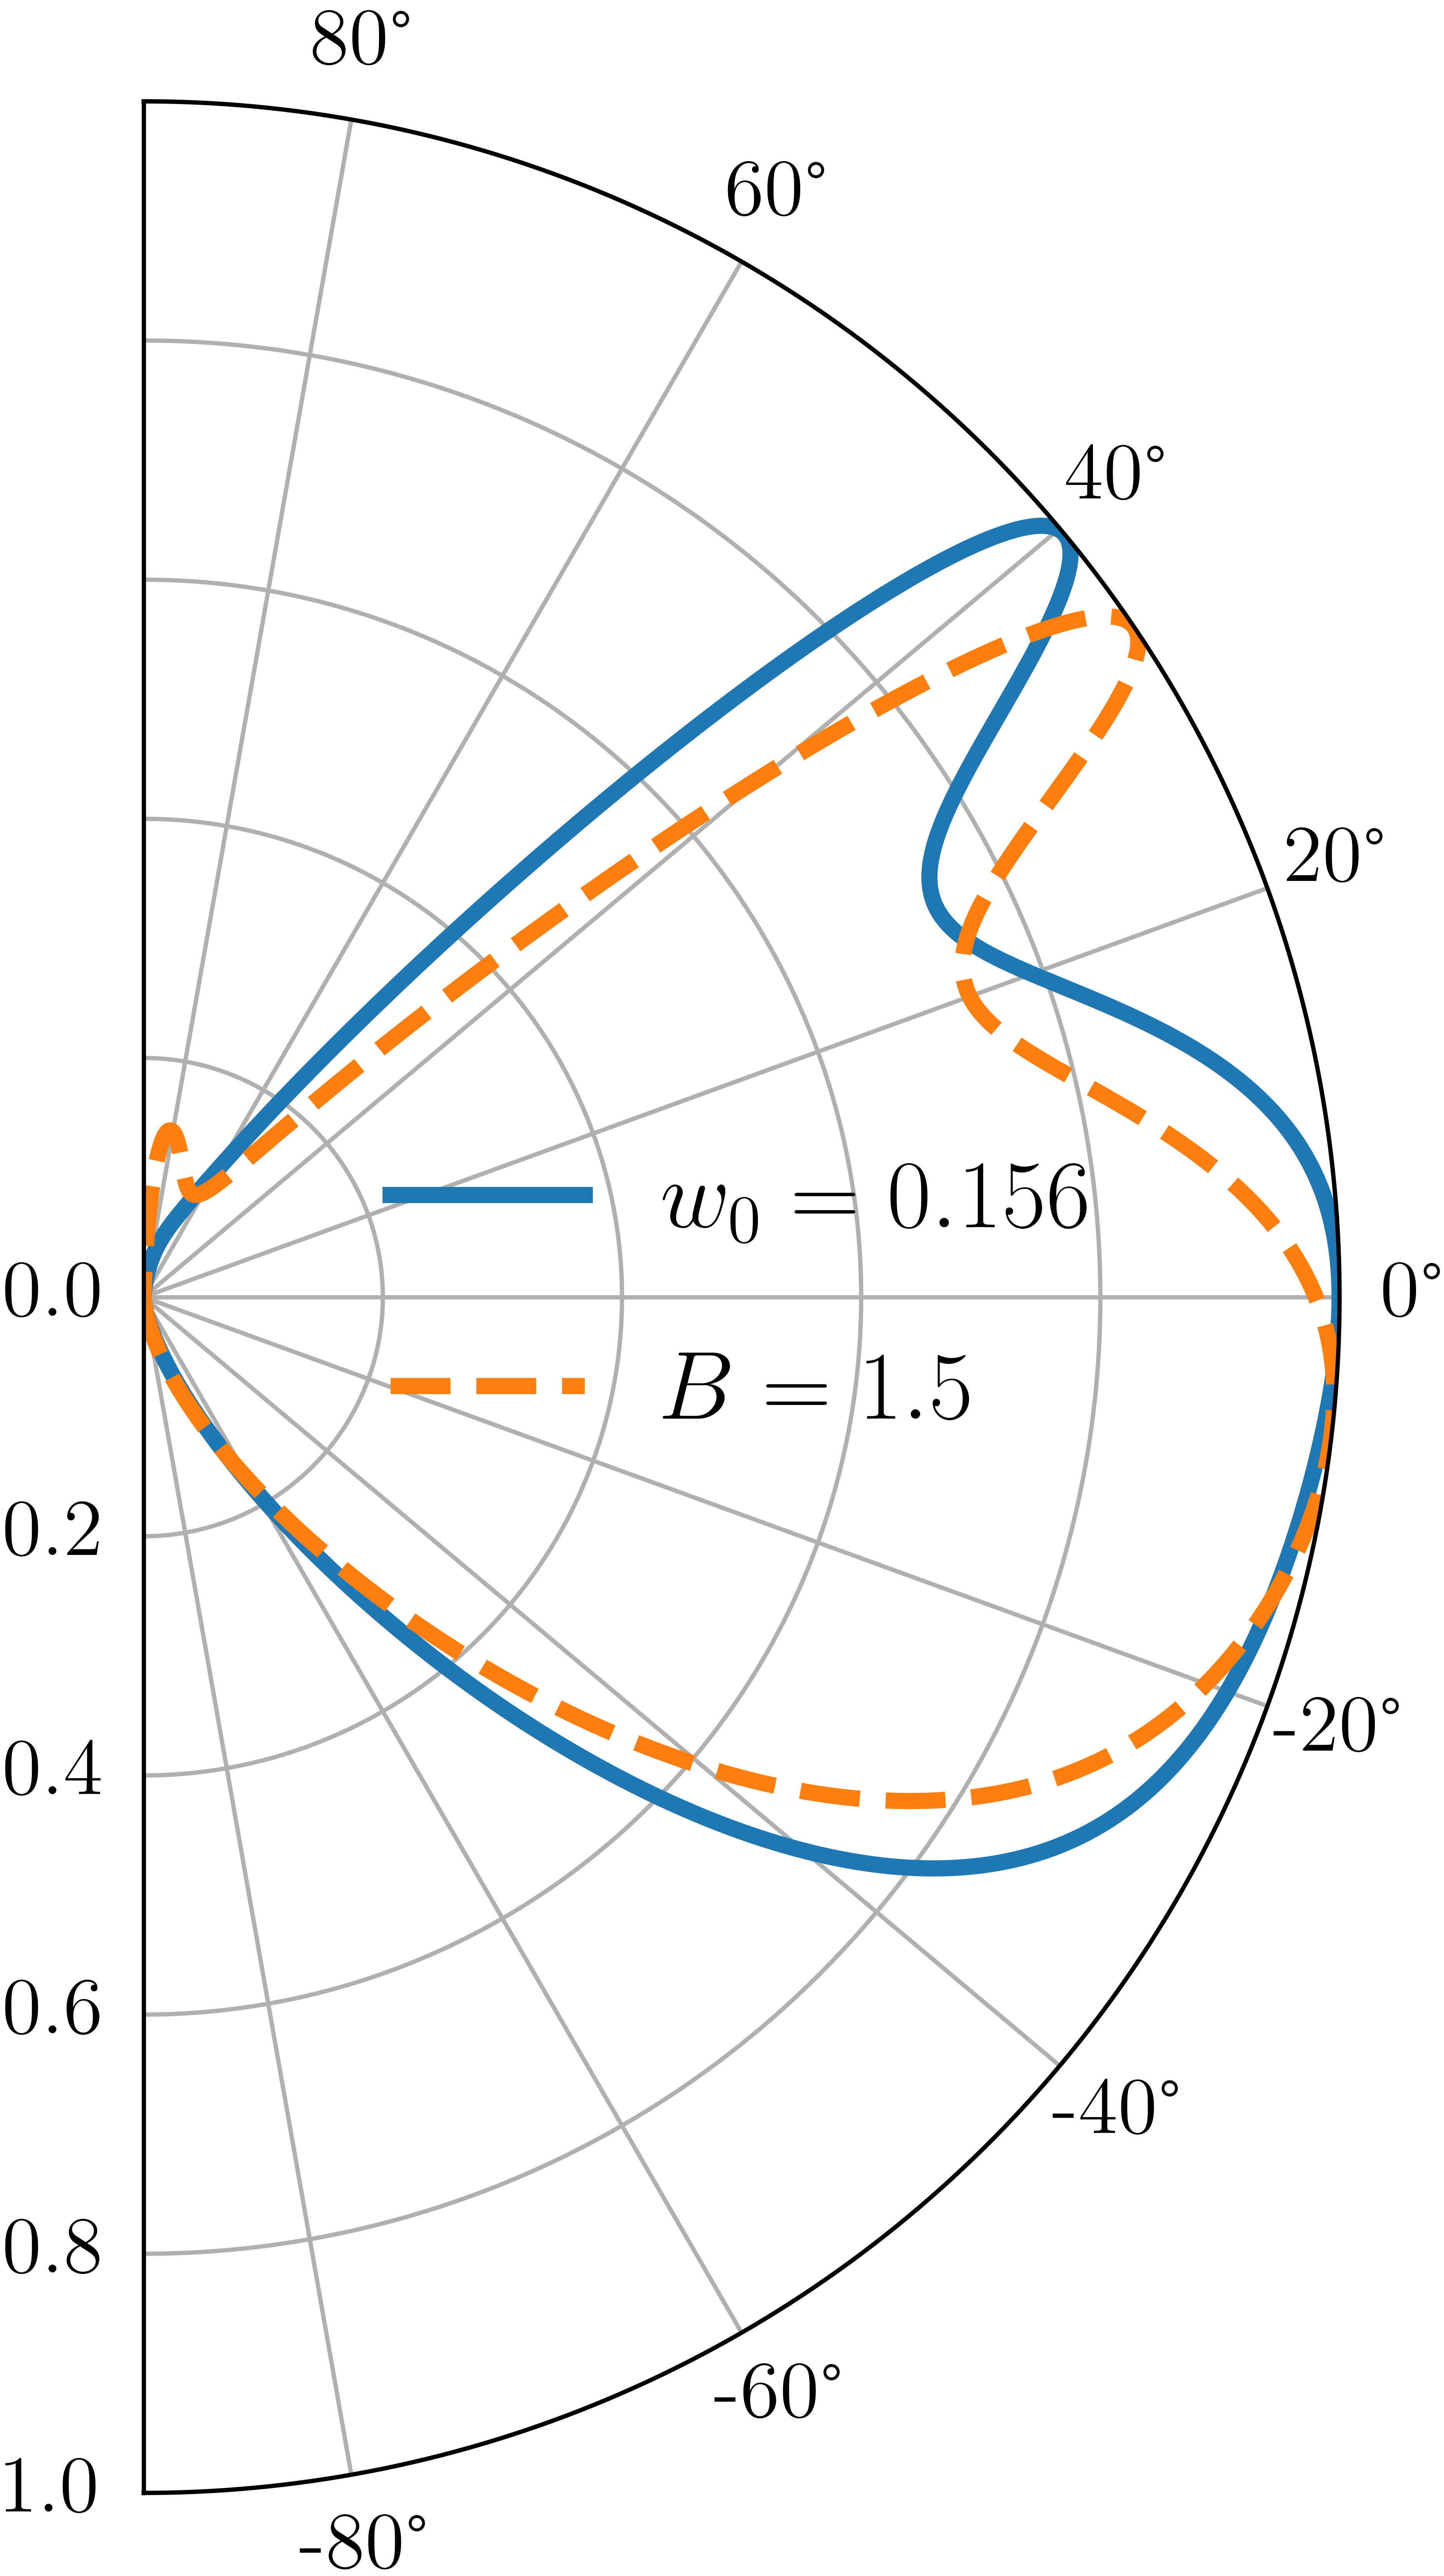
\includegraphics[width=\linewidth]{fig/pseudo B field/Ef0.0832 U0.285 B1.5 w0.156.png}
            \caption{}
            \label{fig:pseudo2}
        \end{subfigure}

        \begin{subfigure}[b]{0.3\linewidth}
            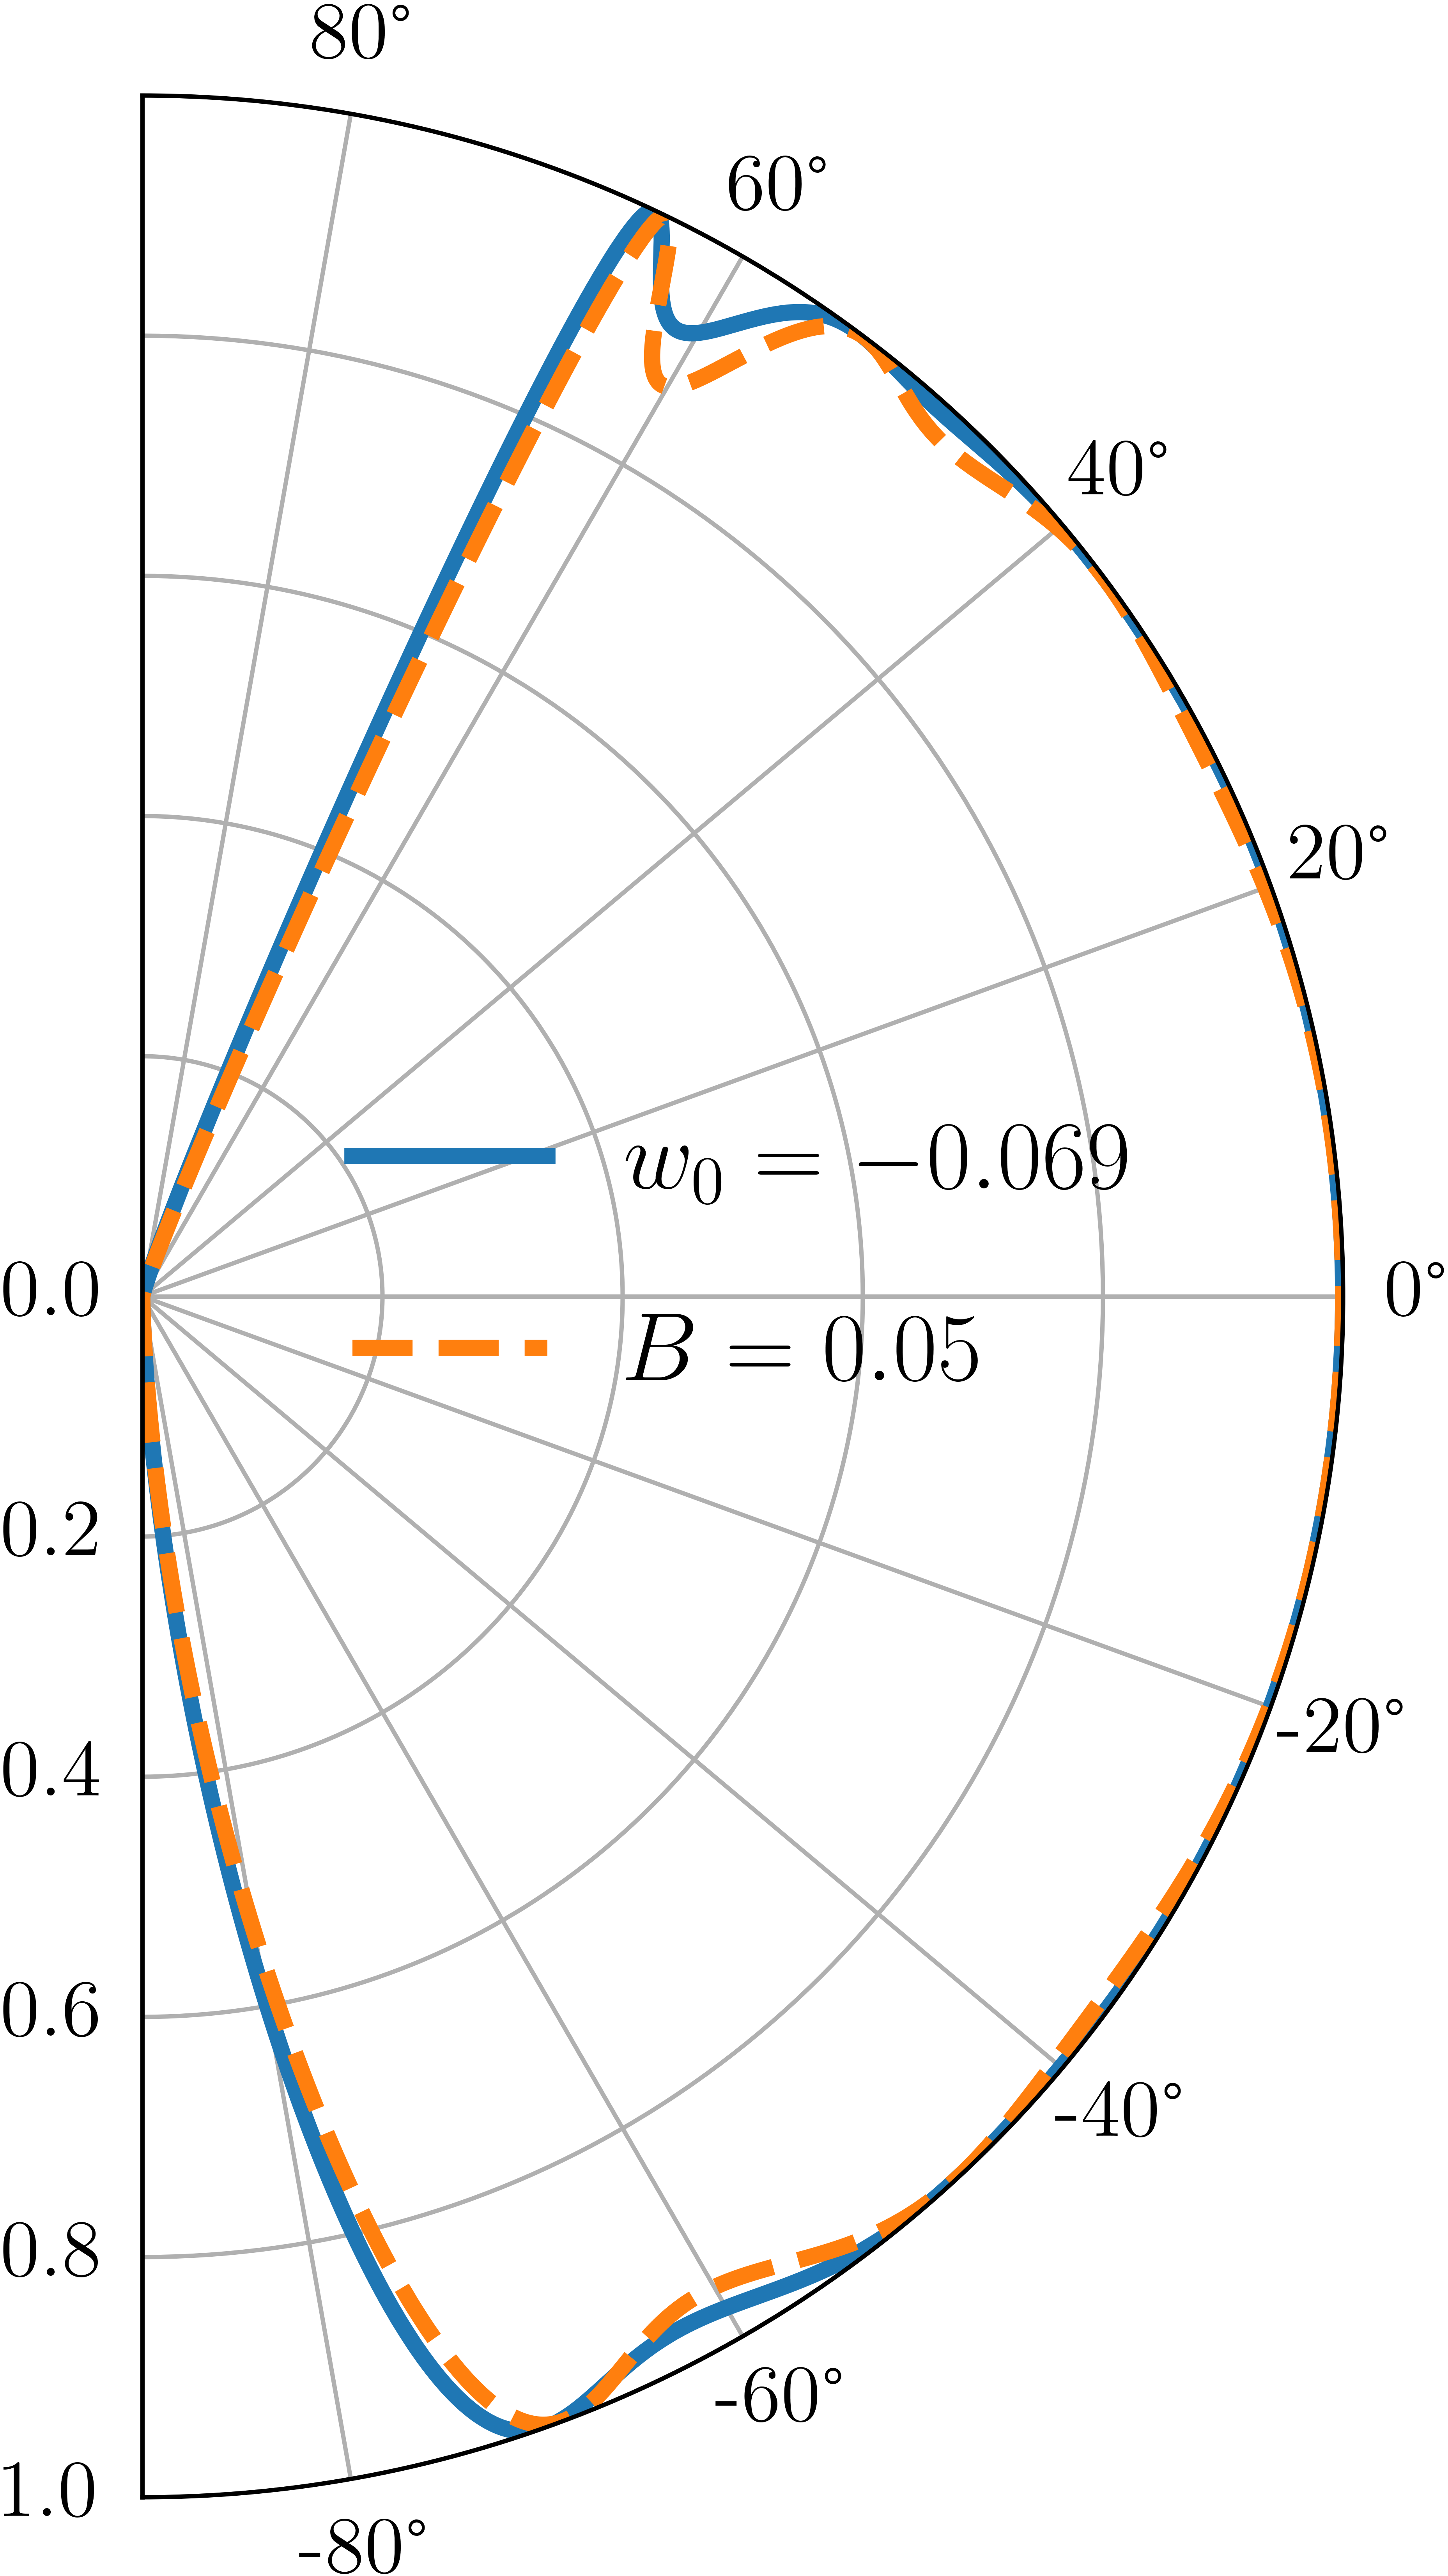
\includegraphics[width = \linewidth]{fig/pseudo B field/Ef0.0832 U0 B0.05 w-0.069.png}
            \caption{}
            \label{fig:pseudo3}
        \end{subfigure}
        \begin{subfigure}[b]{0.3\linewidth}
            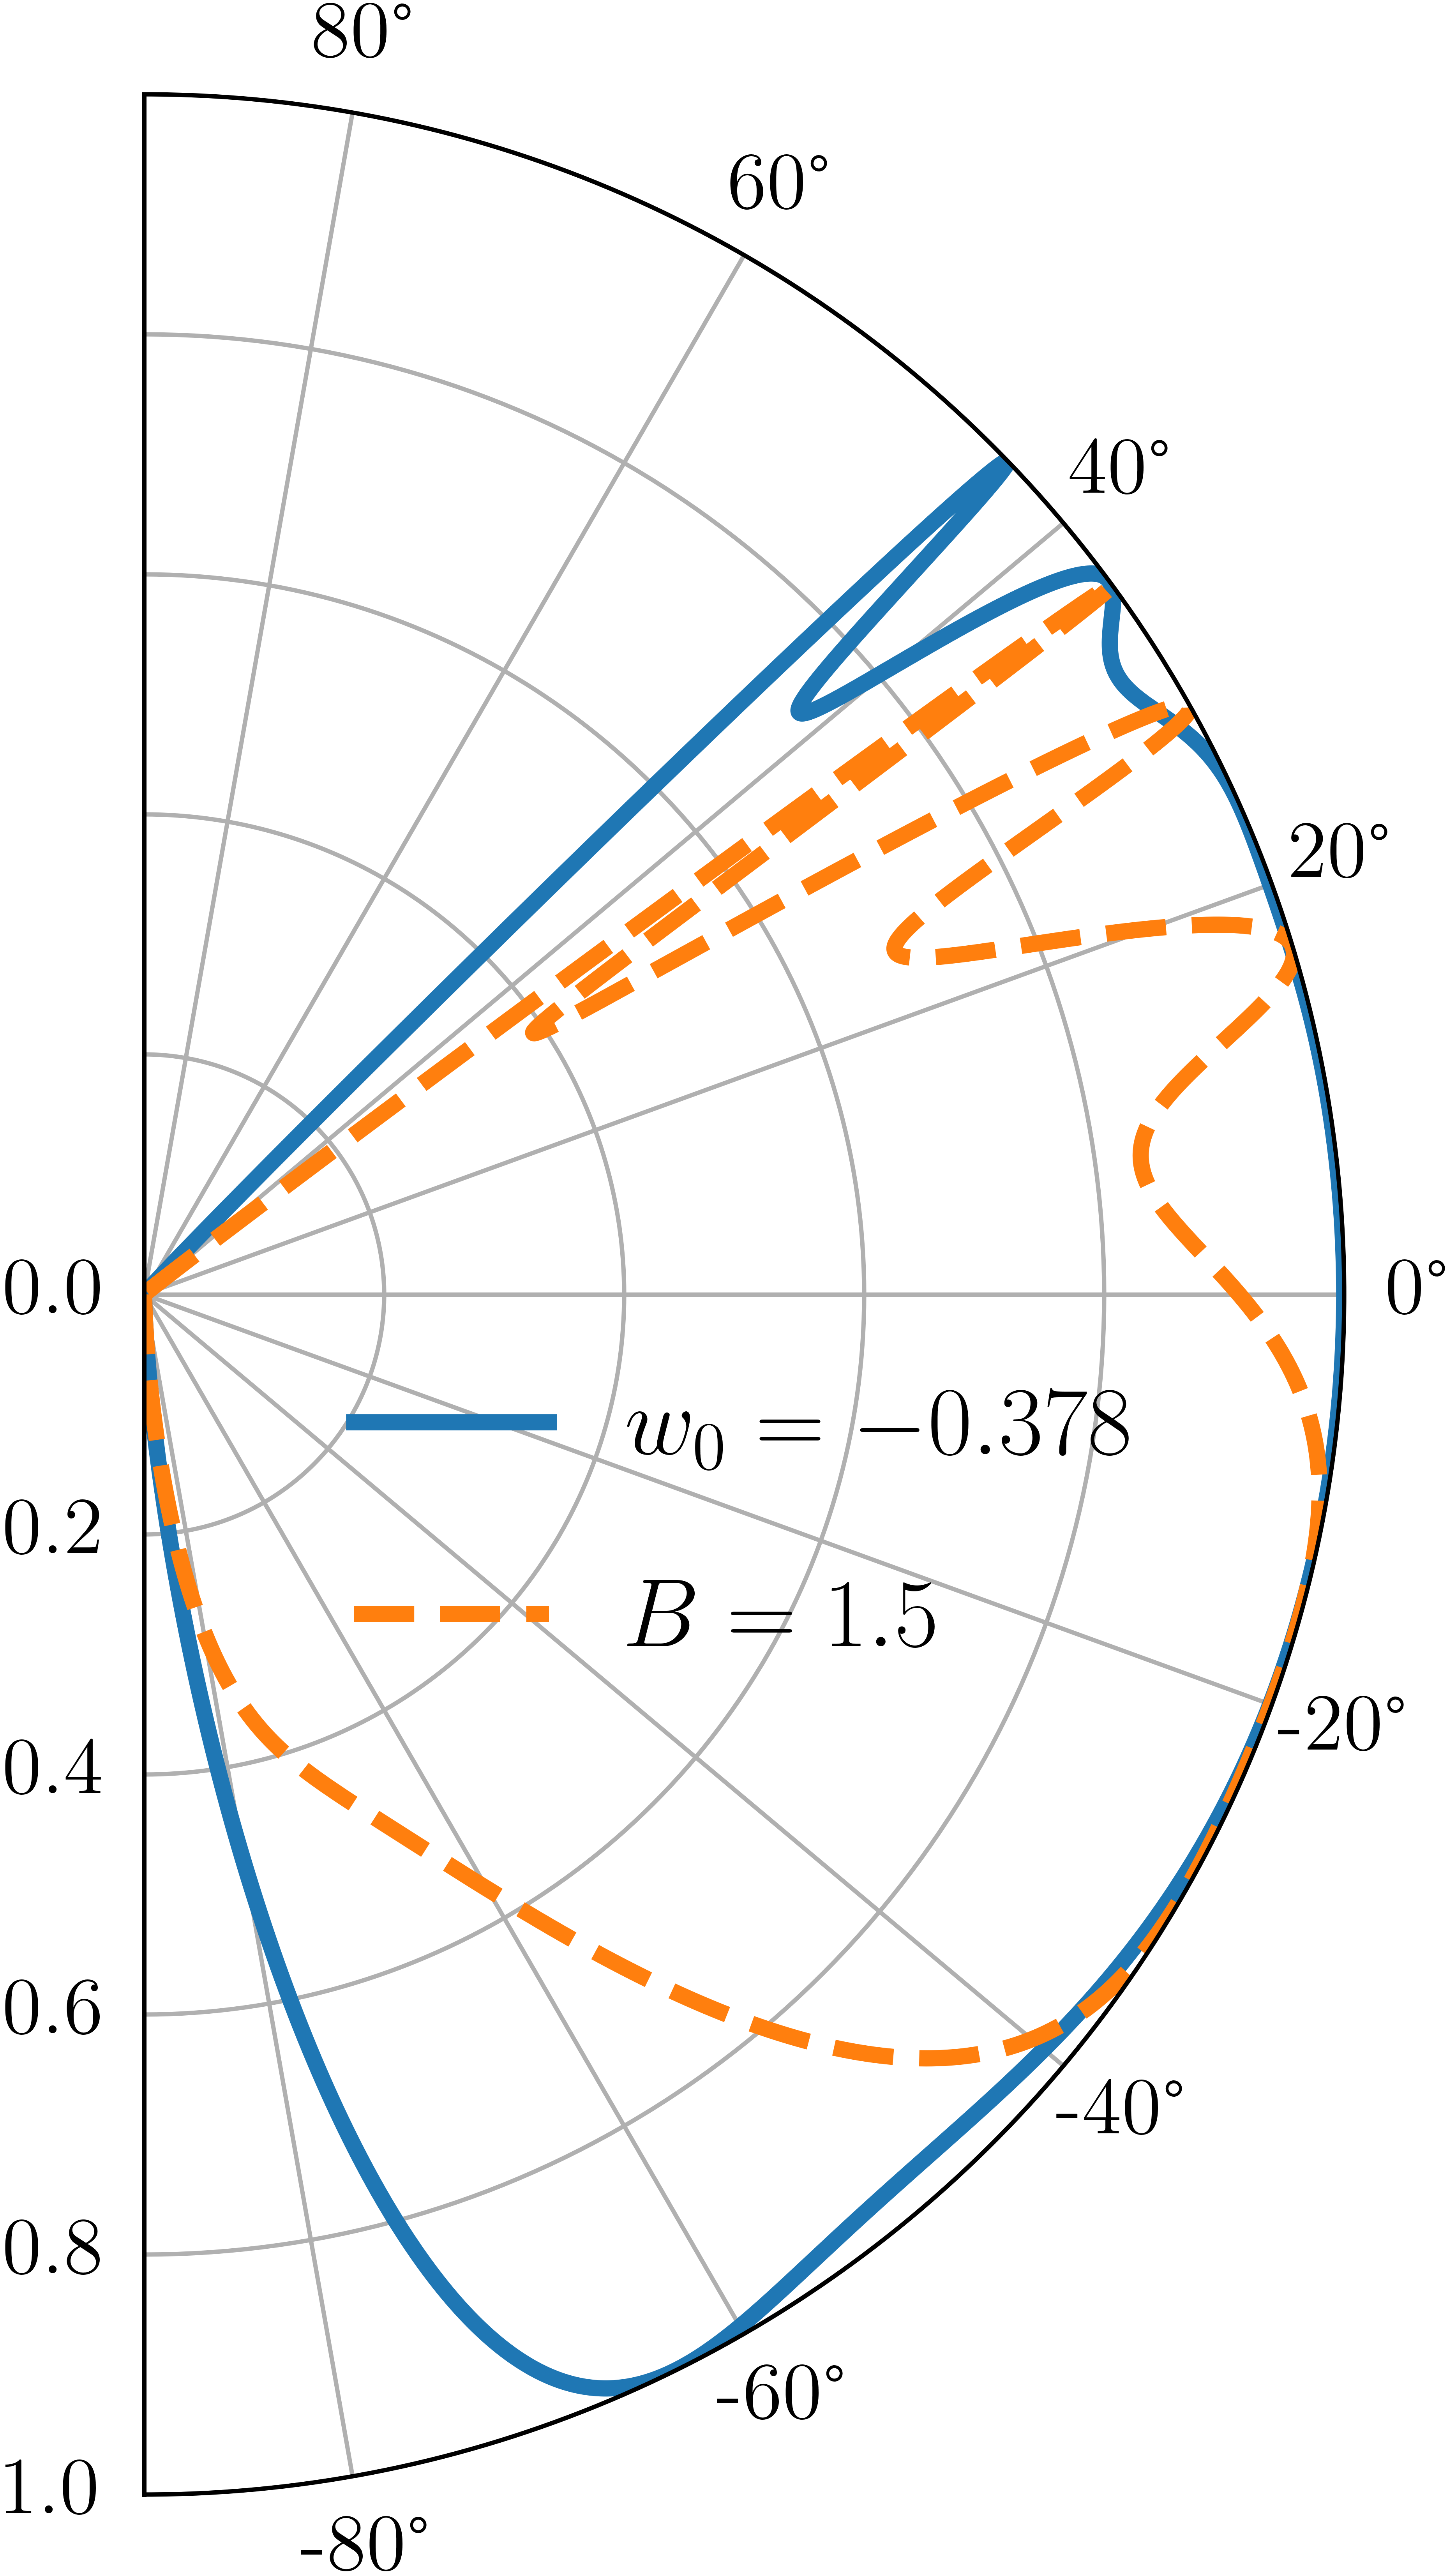
\includegraphics[width = \linewidth]{fig/pseudo B field/Ef0.0832 U0 B1.5 w-0.378.png}
            \caption{}
            \label{fig:pseudo4}
        \end{subfigure}
        \caption{The polar plot of transmission probabilities as a function of incident angle of the system with tilted mismatch Dirac cone 
                (solid line) and non-tilted system under the influence of delta magnetic field (dashed line). The Fermi energy $E_F = 83$ 
                meV is the same for all plot, the gate potential $U = 285$ meV for (a) and (b), $U = 0$ for (c) and (d) }
        \label{fig:pseudo}
    \end{figure}



\section{The key consequence of the mismatch effect}

    The magnetic field strength are related to the magnitude of the tilt.